\chapter{Introduction}
\label{ch:introduction}

\section{Motivation}
\label{sec:motivation_of_thesis}

% Outline
% ECS range
% Questions to be answered
%

% Why climate feedback?
% Why simple model?
% What aims?

Climate feedbacks are the processes in the climate system that can either amplify or dampen its responses to the external perturbations \citep{Bony2006,Soden2006}. Understanding these feedbacks is key to demystify the unresolved problems in climate system. For example, the climate sensitivity, i.e., how the global mean surface temperature change in response to increased greenhouse gas, is one of the central problems in climate change studies \citep[e.g.,][]{Bony2006,Stocker2013,Sherwood2020}, and narrowing down the range of climate feedbacks, especially the range of cloud feedbacks, is crucial to constrain the climate sensitivity \citep[e.g.][]{Cess1990intercomparison,Webb2006contribution,Vial2013,Zelinka2020causes,Myers2021}. Despite the efforts payed by the climate communities, the general circulation models (GCMs) still do not have consensus on the sign of global mean cloud feedback \citep{Zelinka2020causes}, whose uncertainty is still the leading cause of intermodel spread of climate sensitivity \citep{Ceppi2017,Zelinka2020causes}. Therefore, to understand the underlying causes for cloud feedback uncertainty \citep[e.g.,][]{Bony2005,Vial2013,Qu2014,Webb2015,Zelinka2016insights,Geoffroy2017} and to find the potential constraints to it \citep[e.g.,][]{Qu2015positive,Klein2017low,Myers2016,Scott2020,Myers2021,Ceppi2021observational} are key tasks in current climate research.

In addition, it should be noted that the temperature change under global warming are not uniform across the globe, with amplified warming in over polar regions \citep[`polar amplification'; e.g.,][]{Manabe1975,Pithan2014}. It is believed that diminishing sea ice plays a leading role in recent Arctic temperature amplification \citep{Screen2010}. Nevertheless, polar amplification can also occur in simulations even without sea ice \citep[e.g.,][]{Alexeev2005,Cai2005,Cai2006,Langen2012}. In this case, the roles of climate feedbacks are important to understand the temperature changes in polar regions \cite[e.g.,][]{Pithan2014,Kim2018}.

%The global mean surface temperature change in response to increased greenhouse gas, namely the climate sensitivity, is one of the central problems in climate change studies \citep[e.g.,][]{Bony2006,Stocker2013,Sherwood2020}. The estimates of climate sensitivity depend critically on the climate feedbacks, the processes that can either amplify or dampen the responses of climate system to the external perturbations \citep{Bony2006,Soden2006}. 

Therefore, understanding the roles of climate feedbacks is essential to comprehend the possible changes of climate system under global warming, and the goal of this thesis is to understand these radiative feedbacks through the idealized climate models. In doing so, Isca model \citep{Vallis2018}, an intermediate modelling framework developed at University of Exeter, is employed throughout this thesis. Currently there is no sea ice scheme in Isca, so it is impossible to explore the surface albedo feedback with it. But we still can revisit the polar amplification problem with it, only focusing on the roles of other climate feedback processes. Another problem of Isca is that it has no cloud scheme at the beginning of this study, meaning the questions related to cloud feedbacks are not able to be investigated within the framework of Isca. But as the cloud feedbacks are vital for climate sensitivity, one of the central problems of current climate change research,  we plan to construct a simple diagnostic cloud scheme first so that we can examine cloud feedbacks under the same framework. Thereby, the following scientific questions are to be addressed in this thesis:
\begin{enumerate}
    \item What roles do the climate feedback processes play in the polar amplification of surface temperature change in idealized aquaplanet simulations without sea ice and clouds?
    \item Could we build a cloud scheme for idealized GCMs that is simple enough but could grasp the key features of cloud fields?
    \item If so, could the scheme be used to probe the underlying causes of the intermodel spread of cloud feedback in climate models? 
\end{enumerate}
The first question intends to understand the roles of climate feedbacks (except surface albedo and cloud feedbacks) in climate system, while the rest questions focus on the clouds, cloud feedback and its uncertainty through a potential simple cloud scheme.

In this chapter, the background knowledge to understand climate feedback is briefly introduced. \secref{sec:earth_rad_budget} describes the Earth's radiation budget, which is the basis for us to understand the energy balance of climate system. In \secref{sec:climate_fbk_intro}, the framework to understand climate feedback is presented, including its definition and the key individual feedbacks in climate system. In addition, the basic mechanisms of these feedbacks are also summarized in short. As the cloud feedback has the largest uncertainty among all the climate feedbacks in current climate models, the necessary knowledge to understand the cloud feedback is presented in \secref{sec:cre_and_cld_fbk_intro}, including the essential features of cloud radiative effect (\secref{sec:CRE_intro}) and the major mechanisms for cloud feedbacks (\secref{sec:intro_cld_fbk_mechanism}). \secref{sec:cld_scheme_history} briefly reviews the development of cloud parameterization schemes, as this study intends to understand the cloud feedback through a simple cloud scheme. Finally, the outline of whole thesis is described in \secref{sec:thesis_layout}.

\section{The Earth’s radiation budget}
\label{sec:earth_rad_budget}

The Earth's climate is driven by the energy flow into and out of the system. The incoming solar radiation (yellow fluxes in \figref{fig:earth_energy_budget}) reaches the Earth at the top of the atmosphere (TOA), then goes through the atmosphere and arrives at the Earth surface. During this process, approximately two thirds of the shortwave (SW) radiation is absorbed by the Earth surface and atmosphere, and roughly one third of this energy is reflected back to space. The surface and atmosphere are heated by this incoming solar radiation, and they also re-emit the longwave (LW) radiation (purple fluxes in \figref{fig:earth_energy_budget}) to keep a relatively stable temperature. Globally, the annual mean incoming solar radiation flux is about 340 Wm$^{-2}$, the reflected solar radiation flux is around 100 Wm$^{-2}$ and the outgoing longwave radiation (OLR) is close to 240 Wm$^{-2}$ at the TOA for period 2000--2010 \citep{Stephens2012update}. These three components balance with each other, with a small positive imbalance (about 0.6 Wm$^{-2}$) at the TOA. A more recent estimate from \cite{Wild2015} (see their Fig. 1) indicates that the global mean OLR is about 239 Wm$^{-2}$, and the TOA energy imbalance is about 1 Wm$^{-2}$.
%But due to the accuracy of the observation itself, it is hard to track the causes of these imbalance.

\begin{figure}[ht]
	\centering
	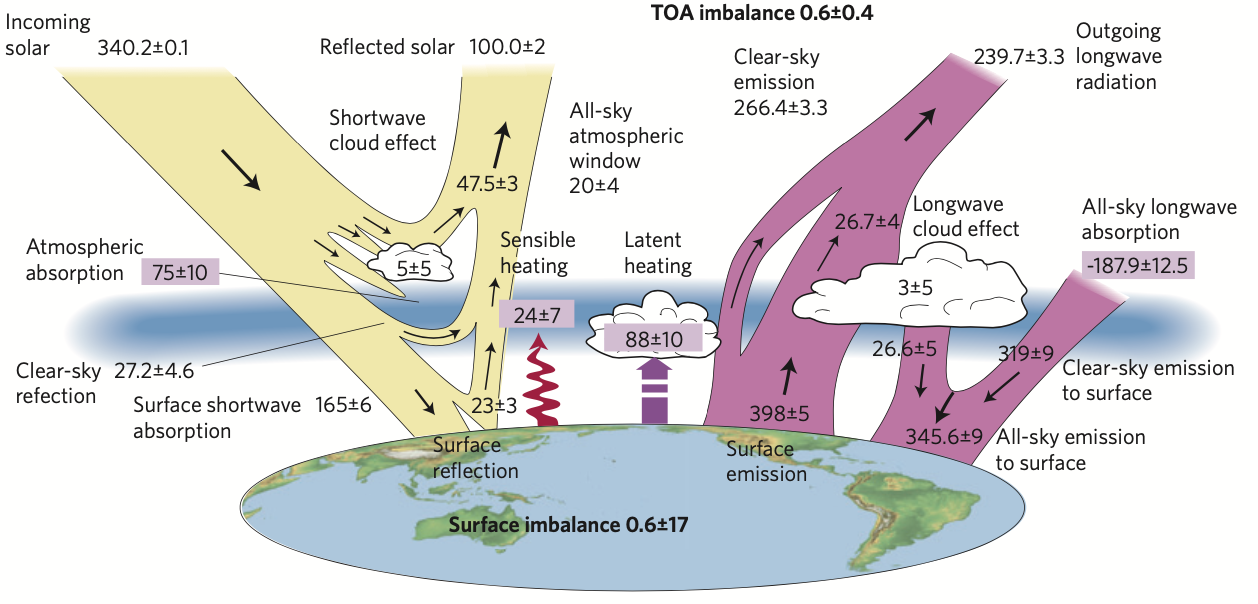
\includegraphics[width=1\linewidth]{{figs/literature_review/earth_enery_budget_Stephens2012}.png}
	\caption[The global annual mean energy budget of Earth for the approximate period 2000–2010 from \cite{Stephens2012update}]{The global annual mean energy budget of Earth for the approximate period 2000–2010. All fluxes are in Wm$^{-2}$. Solar fluxes are in yellow and infrared fluxes in purple. The four flux quantities in purple-shaded boxes represent the principal components of the atmospheric energy balance. Adapted from Fig. B1 of \cite{Stephens2012update}. Reproduced with permission of the Springer Nature.}
	\label{fig:earth_energy_budget}
\end{figure}

As shown in \figref{fig:earth_energy_budget}, the energy budget at the Earth's surface is more complicated than at the TOA. When the incoming solar radiation reaches the surface, the majority (about 165 Wm$^{-2}$) of this solar radiation is absorbed by the surface and only a small portion (about 23 Wm$^{-2}$) is reflected back to space. Of course, these are global mean results and it would be different over certain areas such as Arctic where the surface albedo is large. The global annual mean LW radiation emitted from the surface is about 398 Wm$^{-2}$. Much of this is absorbed by the atmosphere (such as the greenhouse gases, aerosols and clouds), and only a small part (about 20 Wm$^{-2}$) can pass through the atmospheric window region (a portion of the infrared spectrum where there is almost no atmospheric absorption) reaching the TOA directly. The atmosphere can re-emit the absorbed LW radiation both upward and downward, and downward part (about 346 Wm$^{-2}$) can reheat the surface. In addition, due to the temperature and moisture difference between the surface and atmosphere, the surface is also cooled by the latent heat flux (about 88 Wm$^{-2}$) and sensible heat flux (about 24 Wm$^{-2}$) through the turbulent movement of atmosphere. In total, the surface energy budget is balanced by the downward/upward SW and LW radiation, the sensible and latent heat fluxes, but it has much larger uncertainty than at the TOA.

\section{Climate feedback}
\label{sec:climate_fbk_intro}

\subsection{Definition}

\begin{figure}[ht]
	\centering
	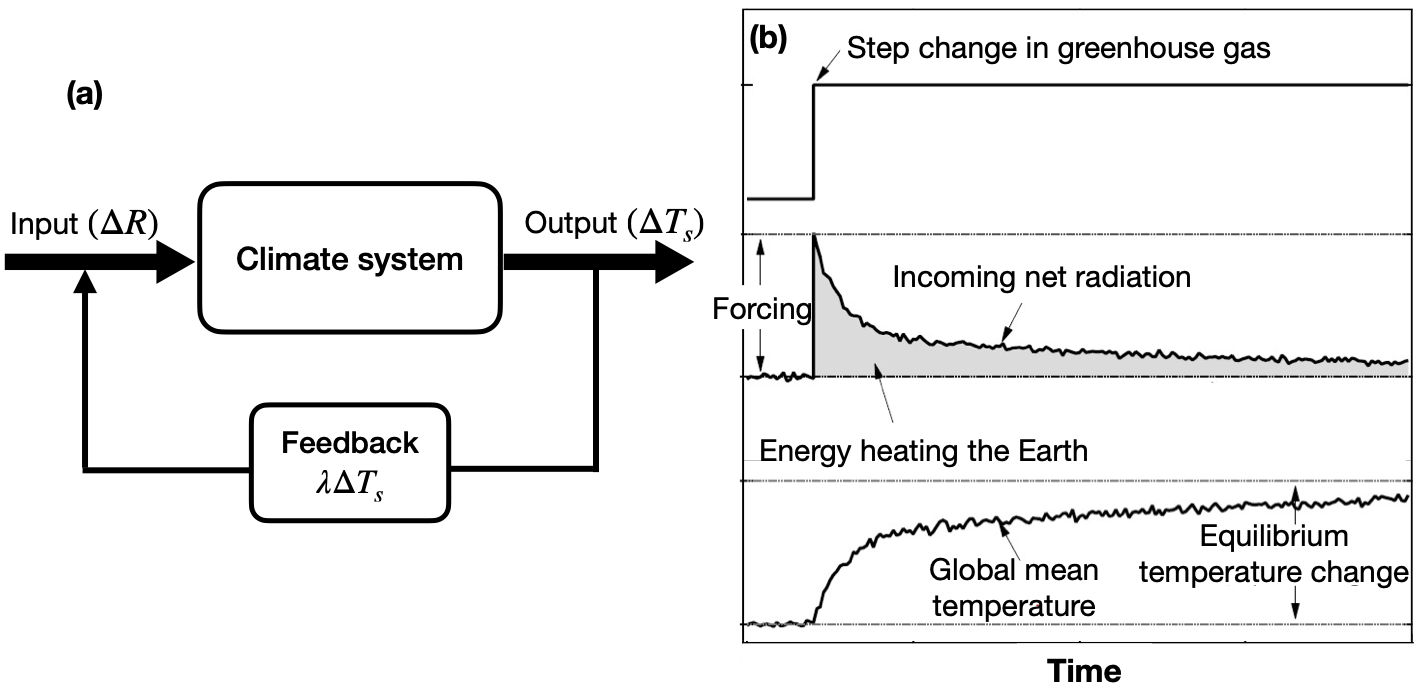
\includegraphics[width=0.95\linewidth]{{figs/literature_review/clim_system_feedback2}.png}
	\caption[Schematic of the forcing and feedback in climate system]{(a) Schematic of feedback in climate system. $\Delta R$ is the input disturbance to the climate system, $\Delta T_s$ is the change of surface temperature and $\lambda$ denotes the climate feedback parameter. (b) The illustration of forcing (middle) and global mean temperature (bottom) change with time due to a step change (top) in greenhouse gas, aerosol, etc. Modified from Fig. 1 of \cite{Murphy2009} with permission of the John Wiley and Sons.}
	\label{fig:schematic_climate_feedback}
\end{figure}

%What is feedback?
 As introduced in \secref{sec:earth_rad_budget}, the energy budget at the TOA is balanced by the incoming solar radiation and the OLR (the imbalance is usually small). Another problem is how to understand the behaviors that the climate system responds to perturbations? In this section, a framework to understand such characters of climate system, including the forcing, feedback, and climate sensitivity will be presented.
 
 In the energy balance model, any disturbance imposed to the system is regarded as the forcing ($\Delta F$), which can be aroused from the perturbation of greenhouse gas concentration (e.g., CO$_2$, CH$_4$), aerosol \citep{Ramanathan2001aerosols}, and change in solar cycle \citep{Frohlich2004solar} or volcanic eruption (\figref{fig:schematic_climate_feedback}). Then climate system will response to this radiative imbalance ($\Delta R$) at the TOA  by changing the surface temperature ($T_s$). As shown in \figref{fig:schematic_climate_feedback}a, the change in surface temperature (i.e. $\Delta T_s$) can in turn impact the radiative balance at the TOA. That is to say the output response is fed back to the system. $\Delta R$ goes to zero when the climate system adjusts towards a new equilibrium (\figref{fig:schematic_climate_feedback}b). Using the idea of feedback\index{Feedback|(}, which is taken from the control system and used to understand the system response to different forcings \citep{Stephens2005cloud},
$\Delta R$ can be linked to the change of surface temperature ($\Delta T_s$) as follows:
\begin{equation}
    \Delta R = \Delta F + \lambda \Delta T_s,
    \label{eq:imbalance_forcing_lambda}
\end{equation}
which can be viewed as a Taylor expansion in surface temperature change ($\Delta T_s$), but neglecting the high order terms \citep{Feldl2013a}. The second term, $\lambda \Delta T_s$, on right hand side reflects the radiative flux change that is linearly depend on the surface temperature change, and $\lambda$ is called the \textit{feedback parameter} \citep{Gregory2004}. At the equilibrium state (i.e., $\Delta R=0$), the total climate feedback is expressed as 
\begin{equation}
    \lambda = -\frac{\Delta F}{\Delta T_s}.
\end{equation}
Thus, $\lambda$ is in units of Wm$^{-2}$K$^{-1}$ and is a measure of the TOA radiative flux change per degree of surface air temperature change. 
% Conceptually, \Eqref{eq:imbalance_forcing_lambda} states that the TOA energy imbalance can be expressed as the sum of the radiative forcing and the radiative response of the system to a global surface temperature anomaly.

%\subsection{Climate sensitivity}
Based on the forcing and feedback analysis framework, the equilibrium climate sensitivity (ECS) \index{Equilibrium climate sensitivity}\index{ECS}, i.e., the equilibrium response of global mean surface air temperature to the radiative forcing from a doubling of CO$_2$ ($F_{2\times}$), can be estimated as:
\begin{equation}
    \text{ECS} = \Delta T_{s\_2\times}=-\frac{F_{2\times}}{\lambda}.
    \label{eq:ecs}
\end{equation}
ECS is a measure of the climate sensitivity of the GCM to the forcing, and has a quite large range ($\sim$1.5--4.5K) among the fifth phase of the Coupled Model Intercomparison Project \citep[CMIP5;][]{Taylor2012overview} models \citep[e.g.,][]{Andrews2012forcing,Ceppi2017}. In addition, such spread (see the first panel in \figref{fig:zelinka_global_mean_fbks}) does not reduce in recent sixth phase of the Coupled Model Intercomparison Project \citep[CMIP6;][]{Eyring2016overview} models \citep{Zelinka2020causes}. Evidence from historical and paleoclimate records perhaps can help narrow down the uncertainty of ECS \citep{Sherwood2020}, but more work still needed to understand the underlying causes of the uncertainty.
%\cite{Sherwood2020} evaluated the Earth's climate sensitivity based on multiple lines of evidence (feedback process understanding and the historical and paleoclimate records), and find that...

\subsection{Individual feedbacks}
\label{sec:individual_fbks}

% Introduction of different feedbacks?
In climate system, climate feedbacks are the processes that can either amplify or dampen the effects of climate forcings \citep{Hansen1984}. A feedback that amplifies the initial perturbation is called a ``positive feedback", while a ``negative feedback" reduces the initial perturbation. In general, $\lambda$ can be decomposed into feedbacks from different physical processes, such as temperature (Planck and lapse rate), water vapor, surface albedo, clouds, etc. These climate feedback parameters can be evaluated as follows
\begin{equation}
    \lambda = \frac{\partial R}{\partial T_s} = \sum_x \frac{\partial R}{\partial x}\frac{\partial x}{\partial T_s} + \text{Re}, %\text{high-order terms},
    %+ \sum_x\sum_y \frac{\partial^2 R}{\partial x\partial y}\frac{\partial x\partial y}{\partial^2 T_s}+\dots 
    \label{eq:lambda}
\end{equation}
where $x$ represent the climate variable such as temperature, water vapor, surface albedo and cloud properties. $\frac{\partial R}{\partial x}$ can be treated as the feedback parameter due to climate variable $x$. When neglecting the nonlinearities and interactions among different feedbacks, the high-order residual term ($\text{Re}$) is usually neglected in analysis. 

The temperature feedback in climate system can be decomposed into Planck and lapse rate feedback \citep{Soden2006}. The Planck feedback \index{Feedback!Planck} \index{Planck feedback}  assumes that the tropospheric temperature change is vertically uniform and equals to the surface temperature change \citep{Bony2006,Soden2006}. In other words, there is no vertical temperature change in the troposphere. The Planck feedback is named due to the Planck's blackbody radiation law, which is the basic and the strongest negative feedback in climate system. According to the Stefan--Boltzmann law, the longwave radiation emitted by the Earth’s surface rises with temperature following $\text{OLR}=\epsilon\sigma T_s^4$, where $\epsilon$ is the surface emissivity close to unity and $\sigma$ ($5.67\times 10^{-8}\, \mathrm{W\, m^{-2}\,K^{-4}}$) is the Stefan--Boltzmann constant \citep{Pithan2014}. Thus, the Planck feedback can be expressed as $\lambda_P = \frac{\partial R}{\partial T_s}=-4\epsilon\sigma T_s^3=-4\frac{\text{OLR}}{T_s}$ (assuming $R$ downward positive). As shown in \figref{fig:earth_energy_budget}, the OLR is closed to 240 Wm$^{-2}$, and the observed global mean surface temperature of Earth is about 288K, thus the estimated Planck feedback is about $\lambda_P=-4\times 240/288\approx -3.3$ Wm$^{-2}$K$^{-1}$, closed to the multi-model mean results from CMIP models (see Planck column in \figref{fig:zelinka_global_mean_fbks}). As the physical law to control the Planck feedback is quite solid, its intermodel spread is the smallest among all the climate feedback parameters in models from the CMIP5 and CMIP6 (see \figref{fig:zelinka_global_mean_fbks}).

% \begin{figure}[ht]
% 	\centering
% 	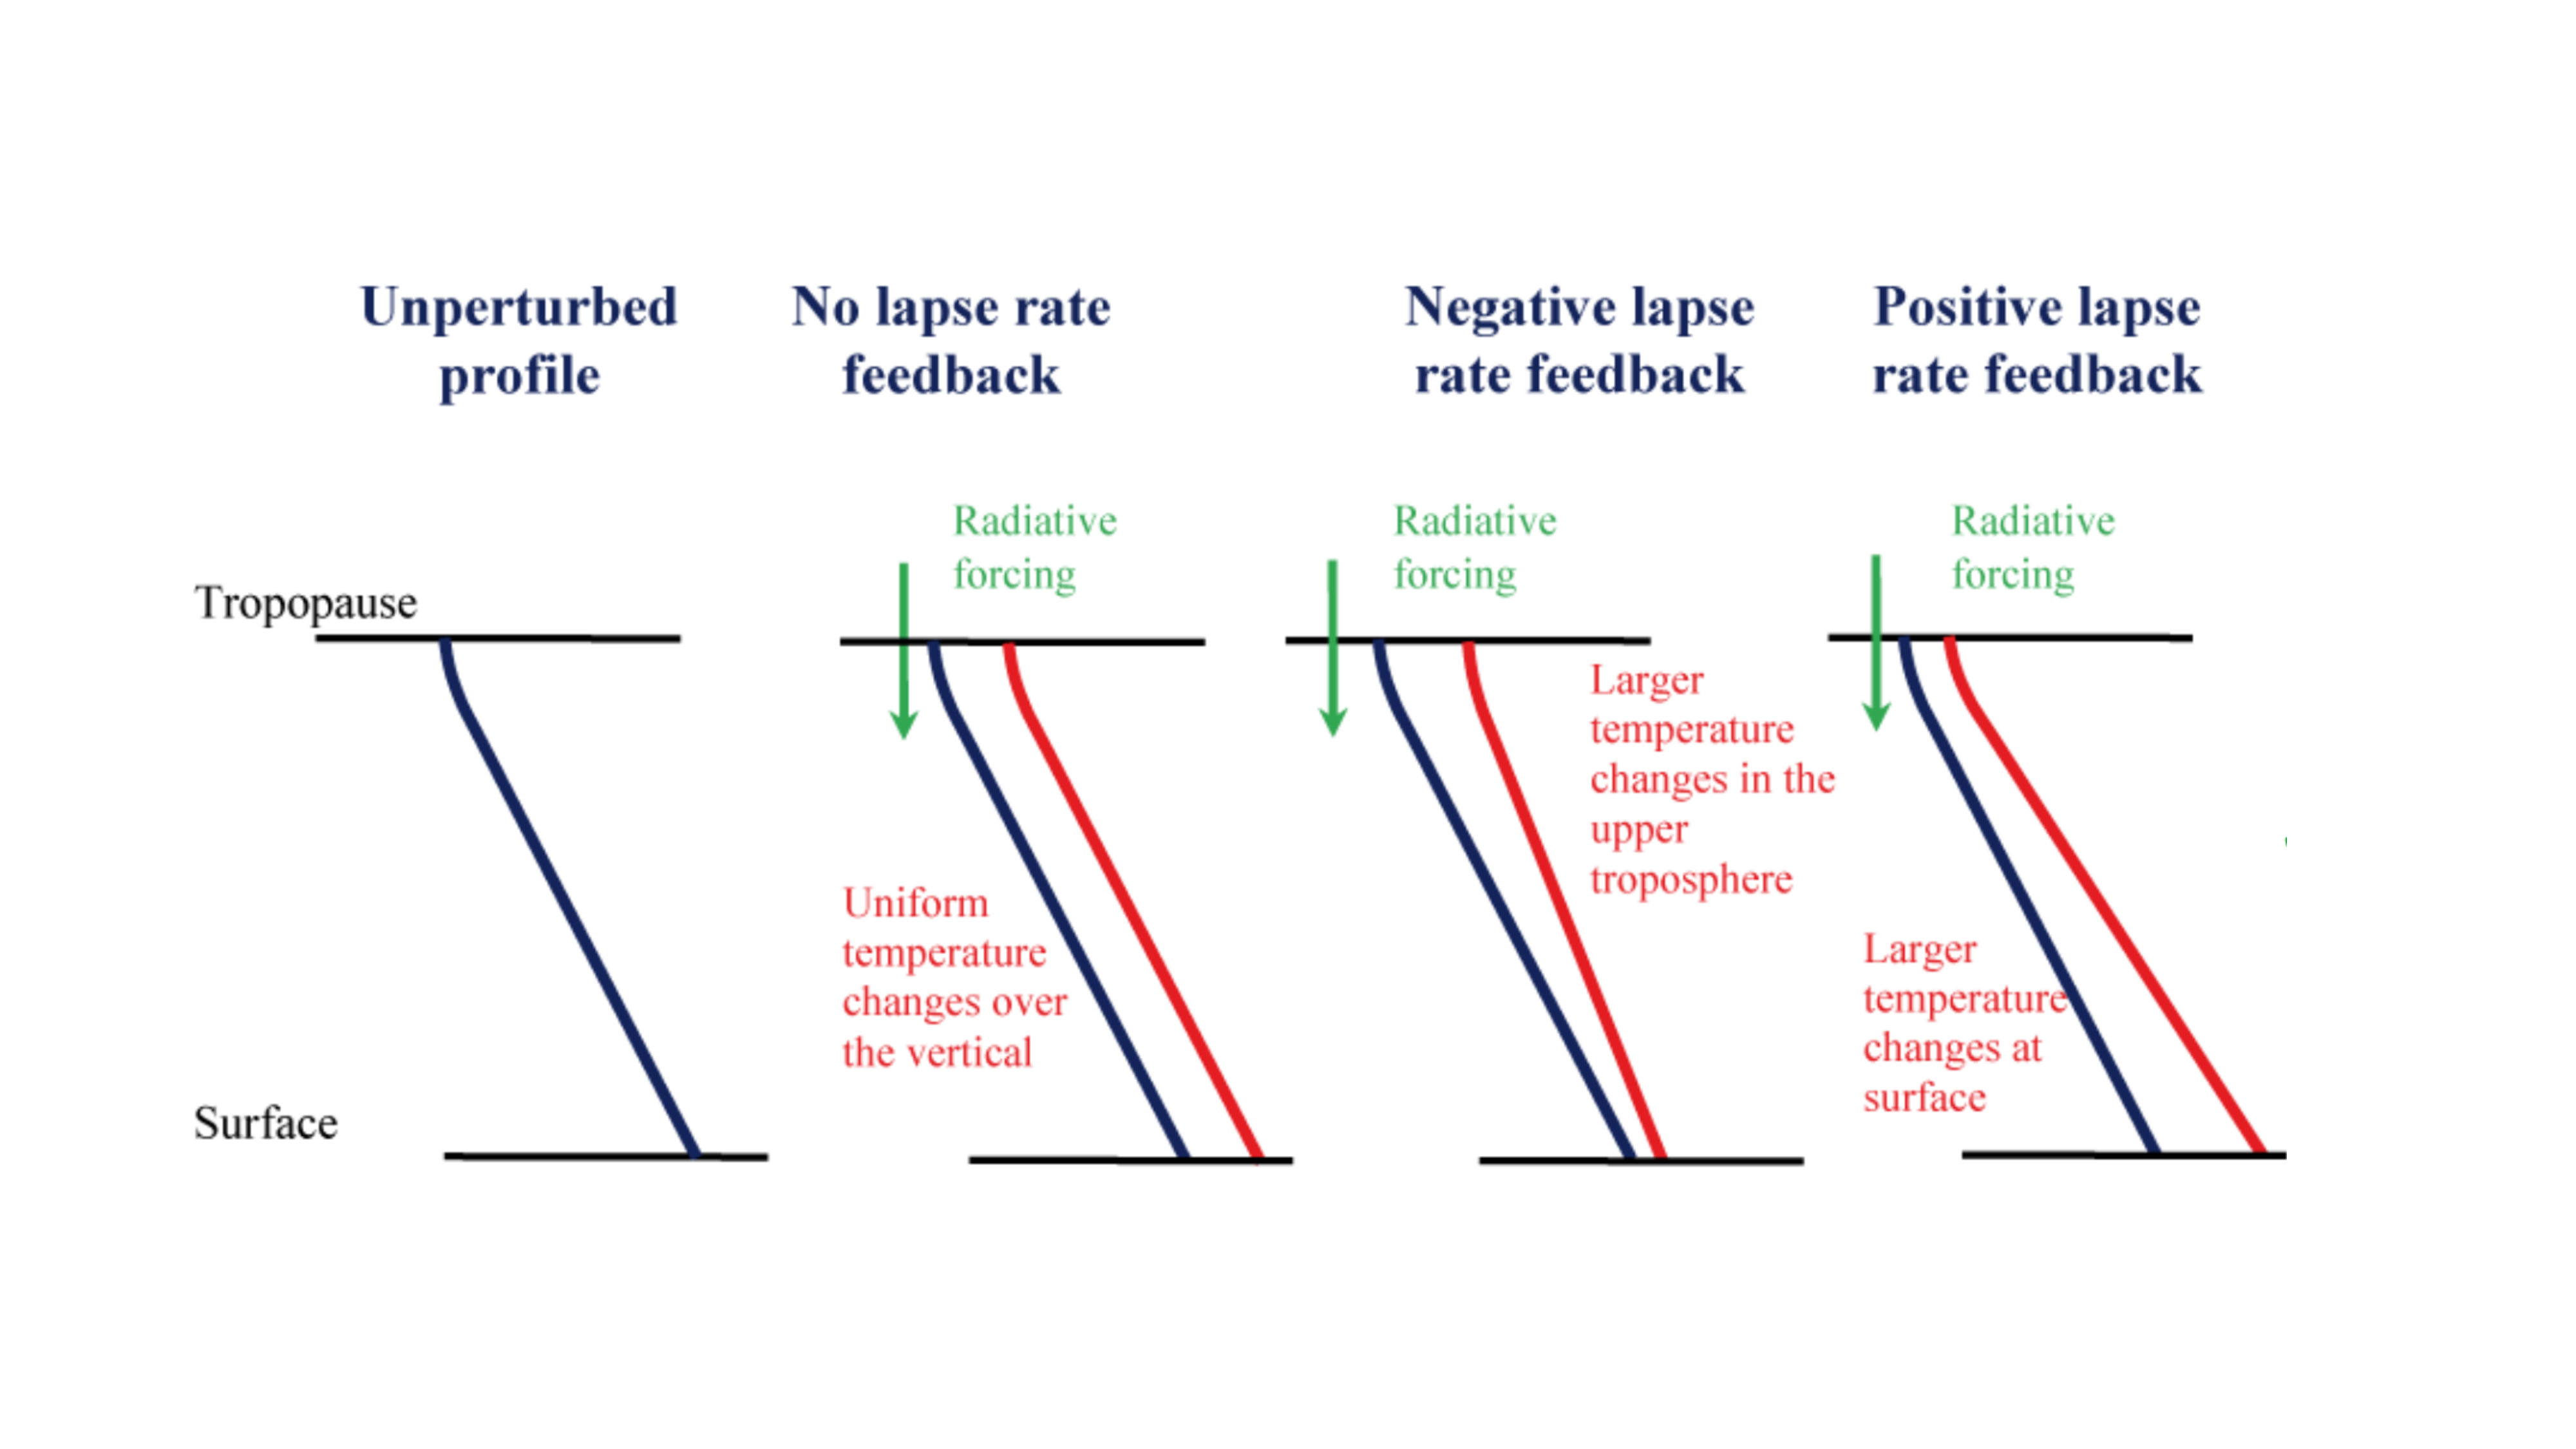
\includegraphics[width=0.95\linewidth]{{figs/literature_review/lapse_rate_fbk}.pdf}
% 	\caption{Schematic representation of positive and negative lapse-rate feedbacks. The dark blue and red lines are for the unperturbed and perturbed temperature profiles in troposphere, respectively. Modified from Fig. 4.10 of \cite{Goosse2010introduction}.}
% 	\label{fig:lapse_rate_fbk_illustration}
% \end{figure}

The lapse rate feedback \index{Feedback!lapse rate} \index{Lapse rate feedback} is associated with the vertical temperature change in troposphere that deviates from the surface temperature change \citep{Bony2006,Soden2006,Feldl2017}. As we know, the atmosphere's temperature decreases with height in the troposphere (the rate of such a change is termed as lapse rate), and the emission of longwave radiation varies with temperature, thus the emitted longwave radiation from inhomogenous warming profiles would be different from the uniform warming cases. For example, if there is an enhanced warming at the upper troposphere in response to the radiative forcing at tropopause, more OLR will be emitted than in an uniform temperature change over the vertical. Therefore, the lapse rate decreases and the system loses more energy, so inducing a negative feedback. This is usually the case in tropical regions \citep[see Fig. 5 of][]{Armour2013time}. In contrast, if the  warming is trapped near surface, the lapse rate feedback can be positive due to the strong inversion, the infrared cooling is less efficient than the homogeneous warming, thus providing a positive feedback. This usually occurs in high latitude regions \citep{Armour2013time,Pithan2014,Goosse2018}. Therefore, the global mean lapse rate feedback depends on the relative magnitude of those two opposite effects. On average, the influence of the tropics dominates, so the global mean lapse rate feedback is relatively negative and the multi-model mean value is about -0.5 Wm$^{-2}$K$^{-1}$ in CMIP5/6 models, as shown in \figref{fig:zelinka_global_mean_fbks} (LR column). 

\begin{figure}[ht]
	\centering
	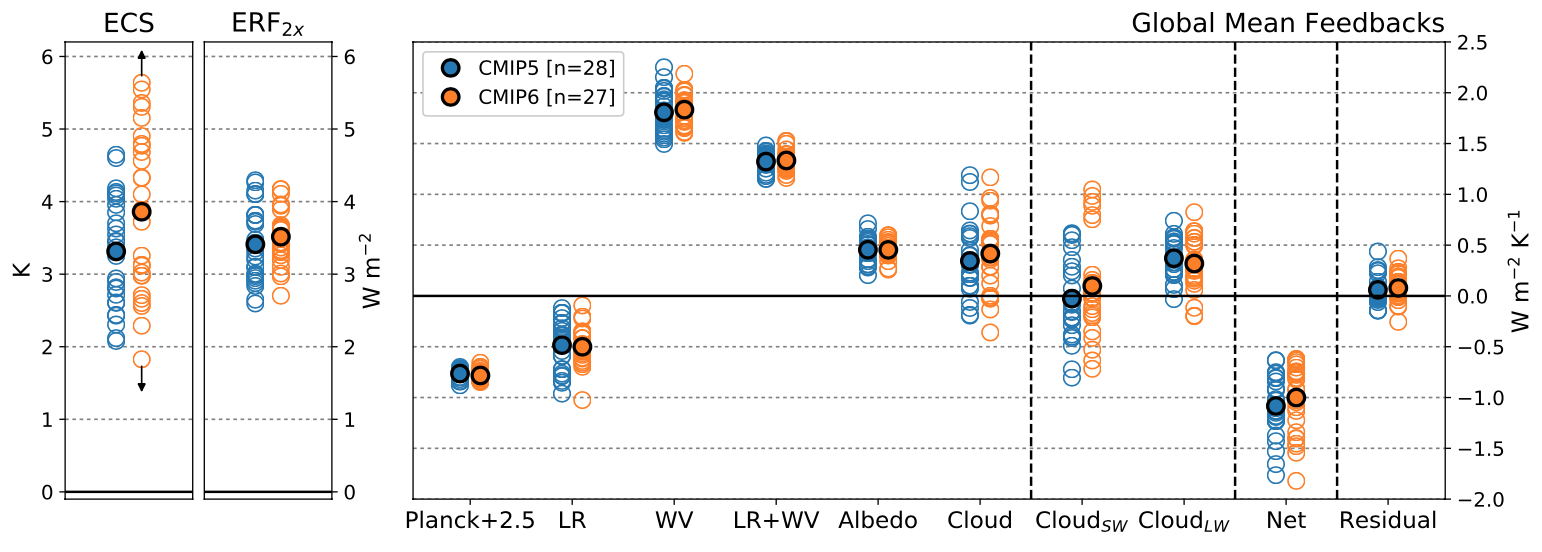
\includegraphics[width=1\linewidth]{{figs/literature_review/global_mean_cld_fbk_cmip56}.png}
	\caption[Equilibrium climate sensitivity (ECS), effective radiative forcing and climate feedbacks from CMIP5/6 models]{Estimates of (left) equilibrium climate sensitivity (ECS), (middle) effective radiative forcing (ERF$_{2\times}$), and (right) global mean climate feedbacks, derived from coupled experiments with abrupt quadrupling of CO$_2$ concentration experiments in CMIP5 (blue dots) and CMIP6 (orange dots) models. The black circles indicate the multi-model ensemble mean values. For display purpose, the Planck feedbacks have been added 2.5 Wm$^{-2}$K$^{-1}$ before plotting. LR and WV are lapse-rate and water vapor feedbacks, respectively. Taken from Fig. S3 of \cite{Zelinka2020causes} with permission of the John Wiley and Sons.}
	\label{fig:zelinka_global_mean_fbks}
\end{figure}

%\subsubsection{Water vapor feedback}
According to the Clausius--Clapeyron relation, the saturated vapor pressure is a quasi-exponential function of temperature. In addition, observations and numerical experiments consistently show that the relative humidity tends to remain more or less constant in response to climate change \citep{Held2000water,Soden2006,Goosse2010introduction}. Thus the warming will cause a significant increase in the amount of water vapor in atmosphere. Since water vapor is the dominant greenhouse gas in the atmosphere \citep{Held2000water}, the increase in water vapor content warms the atmosphere further, which in turn makes the atmosphere hold more water vapor. Thereby, water vapor feedback \index{Feedback!water vapor} \index{Water vapor feedback} is a very strong positive feedback and the multi-model mean value of global mean water vapor feedback in CMIP5/6 models is about 1.8 Wm$^{-2}$K$^{-1}$ (see WV column in \figref{fig:zelinka_global_mean_fbks}).

Despite the large intermodel differences in lapse rate and water vapor feedbacks, the spread in net contribution of both feedbacks is much smaller compared to their individual spread (see LR+WV column in \figref{fig:zelinka_global_mean_fbks}). As pointed by previous studies, the lapse rate feedback and water vapor feedback are closely anti-correlated with each other \citep{Soden2006,PoChedley2018}. \cite{Soden2006} have shown that the models exhibit a nearly constant relative humidity behavior under global warming, suggesting that most of the intermodel spread in water vapor feedback does not step from the various response of relative humidity field, but from differences in the lapse rate response between models. As temperature and water vapor changes are tightly coupled in models, it is better to combine the lapse rate and water vapor feedbacks together when considering sources of intermodel spread in feedback strength \citep{Soden2006,PoChedley2018}. Another option, proposed by \cite{Held_Shell2012}, is to compute Planck and lapse rate feedbacks assuming relative rather than absolute humidity is constant, and a small feedback from changes in relative humidity quantified separately. This method can remove the cancellation between water and lapse rate feedbacks in models, so that the individual feedbacks have less scatter than in the traditional decomposition (see their Fig. 1 in \citealt{Held_Shell2012}; also see their Fig. 1 and Fig. S3 in \citealt{Zelinka2020causes}).

%\subsubsection{Surface albedo feedback}
Surface albedo feedback \index{Feedback!surface albedo} \index{Surface albedo feedback} is related to the regions with snow and ice, which is a positive feedback that enhances climate change \citep{Winton2006surface,Goosse2018}. The mechanism is easy to understand: Warmer temperatures lead to the retreat of snow and ice, which makes the surfaces be less reflective than previous ones. This further causes an increase in the absorbed solar radiation and thus leads to more warming. The global mean surface albedo feedback is weak positive, and the multi-model mean of globally averaged value in CMIP5/6 models is about 0.5 Wm$^{-2}$K$^{-1}$ (see Albedo column in \figref{fig:zelinka_global_mean_fbks}).

% Cloud feedback
\begin{figure}[ht]
	\centering
	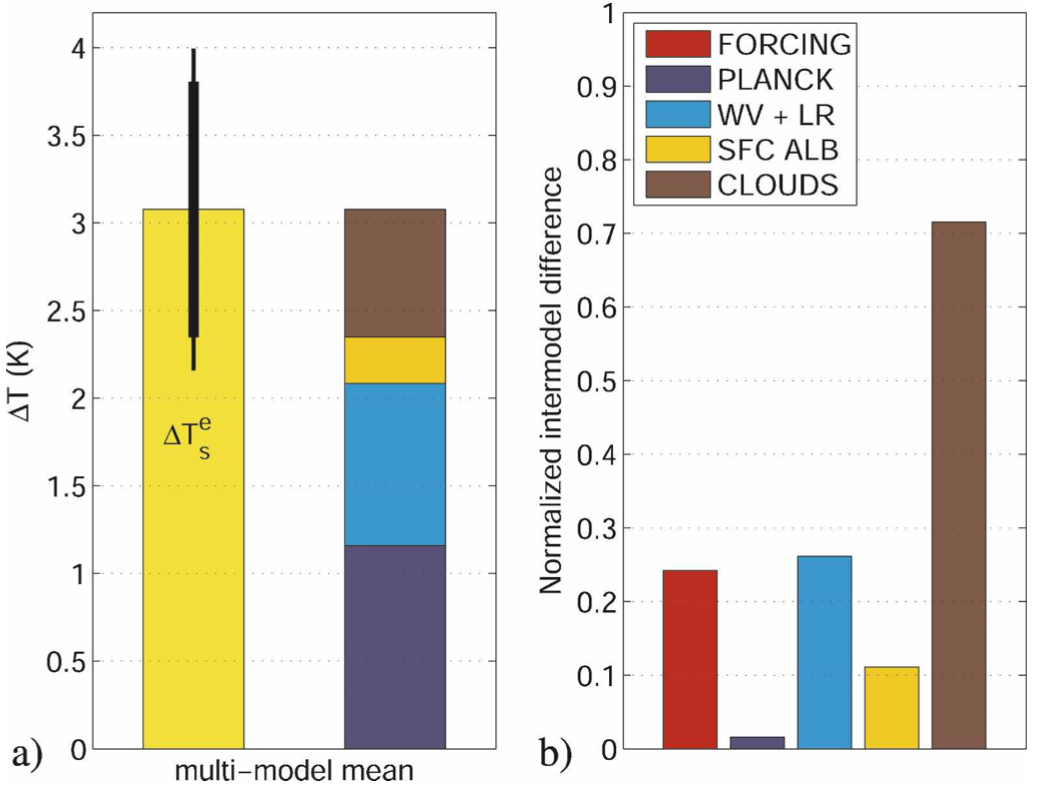
\includegraphics[width=0.6\linewidth]{{figs/literature_review/ECS_contributions}.png}
	\caption[Contributions to ECS and its spread from forcing and different climate feedbacks]{For a CO2 doubling, (a) multi-model mean $\pm$1 standard deviation (thick line) and 5\%–95\% interval (thin line) of the equilibrium temperature change ($\Delta T^e_s$), and contributions to this temperature change associated with the Planck response, combined water vapor and lapse rate (WV+LR) feedback, surface albedo feedback, and cloud feedback. (b) Intermodel standard deviation of the temperature change estimates associated with the radiative forcing, the Planck response, and the various feedbacks normalized by the intermodel standard deviation of the equilibrium temperature change $\Delta T^e_s$ reported in (a). Taken from Fig. 1 of \cite{Dufresne2008assessment}.}
	\label{fig:ECS_contribution_from_fbks}
\end{figure}

Cloud feedback\index{Cloud feedback} is the variation of cloud radiative effect at the TOA in response to global warming. In the fifth assessment report (AR5) of the Intergovernmental Panel on Climate Change (IPCC), the sign of net cloud radiative feedback is likely positive with an estimate of 0.6 Wm$^{-2}$K$^{-1}$, which, however, has a lot of uncertainties (-0.2 to 2 Wm$^{-2}$K$^{-1}$) \citep{Stocker2013}. A recent estimate of net cloud feedback from CMIP6 models is 0.45 Wm$^{-2}$K$^{-1}$ \citep{Zelinka2020causes,Sherwood2020}, but the intermodel spread has no clear reduction from CMIP5 models (see Cloud column in \figref{fig:zelinka_global_mean_fbks}). Nevertheless, there is still no agreement on the signs of global mean net cloud feedbacks in CMIP5/6 models, and several models show the negative global mean values. Furthermore, the sign disagreements also exist in the shortwave and longwave components of cloud feedback, and such a disagreement is more evident in cloud shortwave component (see Cloud$_{SW}$ and Cloud$_{LW}$ columns in \figref{fig:zelinka_global_mean_fbks}). Cloud feedback is the single largest contributor to the uncertainty in the global mean net climate feedback parameters, and also contributes most to the intermodel spread of ECS \citep{Bony2005,Soden2006,Dufresne2008assessment,Colman2011tropospheric,Vial2013,Ceppi2017,Zelinka2020causes,Sherwood2020}. For instance, \figref{fig:ECS_contribution_from_fbks}b, taken from \cite{Dufresne2008assessment}, quantified the contributions to intermodel difference of ECS from various factors, and found the cloud feedback (brown bar) is the largest source (including forcing) of such uncertainty, although it is not the largest contributor to the multi-model mean of ECS (\figref{fig:ECS_contribution_from_fbks}a). Recently, lots of efforts have been paid trying to narrow down the range of ECS by finding possible observational constraints on cloud feedbacks \citep[e.g.,][]{Cesana2021,Myers2021}. The next questions are why the intermodel spread of cloud feedback is so large, and what mechanisms control the cloud response to global warming, as to be reviewed in next section. \index{Feedback|)}

%Moreover, cloud feedback is the largest uncertainty of simulated climate response to CO$_2$ foricng (i.e. climate sensitivity) in GCMs \citep{Ceppi2017,Zelinka2020causes}

%its uncertainty still the largest among all the feedback parameters (see Table 1 of \citealt{Sherwood2020}) and
%As shown in Figure \ref{fig:zelinka_global_mean_fbks}, comparing to other feedback parameters, cloud feedback has the largest intermodel spread, and is the largest uncertainty of simulated climate response to CO$_2$ foricng (i.e. climate sensitivity) in GCMs \citep{Ceppi2017,Zelinka2020causes}.

% As our understanding in cloud related processes is limited, the representation of clouds in general circulation models (GCMs) is still full of uncertainties. Moreover, the interaction between clouds and other physical parameterization schemes, and the coupling between clouds and circulation, 

%\section{Clouds and cloud radiative effect}
\section{Cloud radiative effect and cloud feedback}
\label{sec:cre_and_cld_fbk_intro}

\subsection{Cloud radiative effect}
\label{sec:CRE_intro}

To answer the questions proposed at the end of last section, the basic knowledge about clouds and their roles in climate system are briefly introduced first.

\begin{table}[htp]
\centering
\small %\scriptsize
\caption{Statistics of the annually averaged total cloud amount (\%) for various regions, which are from the ISCCP H-series data sets \citep{Young2018} from 1984 to 2014.}
\vspace{0.5em}
\begin{tabular}{cccc}
	\toprule
	Region & Ocean & Land &  Total\\
	\midrule
	Global & 71.7 & 54.8 & 66.1 \\
	15$^\circ$S -- 15$^\circ$N &  62.4&  63.5& 62.6 \\
	15$^\circ$N -- 35$^\circ$N &  60.1&  46.6& 55.2 \\
	15$^\circ$S -- 35$^\circ$S &  65.0&  48.3& 61.4 \\
	35$^\circ$N -- 60$^\circ$N &  80.9&  64.6& 72.5 \\
	35$^\circ$S -- 60$^\circ$S &  84.0&  65.0& 83.5 \\
	60$^\circ$N -- 90$^\circ$N &  68.9&  62.0& 66.5 \\
	60$^\circ$S -- 90$^\circ$S &  80.1&  44.3& 60.1 \\
	\bottomrule
\end{tabular}
\label{tab:statistics_cld_amt}
\end{table}

Clouds usually cover more than half areas of the Earth at any given time \citep{Houze2014,Ramanathan1989}, which is supported by recent International Satellite Cloud Climatology Project (ISCCP) H-series products \citep{Young2018}, as shown in \tabref{tab:statistics_cld_amt}. Although the cloudiness varies among different regions, the annual mean cloud amount is usually larger than or close to 50\% at any selected region. Also, the cloud amounts are usually larger over ocean regions than over lands (\tabref{tab:statistics_cld_amt} and \figref{fig:cldamt_isccp}d), as the ocean provides an abundance of water vapor. The spatial pattern of cloud climatology is shown in \figref{fig:cldamt_isccp}, and their features is to be discussed in detail in comparison with CRE patterns. Clouds play important roles in Earth's radiation budget and hydrological cycle, and this thesis will focus on their effect on radiation.

As shown in \figref{fig:earth_energy_budget}, clouds can exert competing influences on the energy budget of the Earth. Specifically, clouds cool the Earth by reflecting the incoming shortwave radiation emitted by the sun, and warm the planet by trapping the longwave radiation emitted by the Earth. In general, we quantify the impact of clouds on planet's radiation budget using cloud radiative effect \index{Cloud radiative effect} (CRE)\index{CRE}, which is defined as the differences in TOA net radiative fluxes between all-sky and clear-sky conditions, or the upward radiative fluxes at TOA between clear-sky and all-sky conditions \citep[e.g.,][]{Ramanathan1989,Soden2004,Soden2008,Li2017}. Note that the CRE is also called cloud radiative forcing (CRF) in some literatures \citep[e.g.,][]{Ramanathan1989}, but CRE is more commonly used currently, so we prefer using CRE in this study. According to the definition, the shortwave and longwave CREs at TOA can be computed as follows:
\begin{equation}
    \mathrm{SWCRE} = \mathrm{SW}_{clr}^{\uparrow} - \mathrm{SW}_{all}^{\uparrow},
    \label{eq:swcre}
\end{equation}
\begin{equation}
    \mathrm{LWCRE} = \mathrm{LW}_{clr}^{\uparrow} - \mathrm{LW}_{all}^{\uparrow},
    \label{eq:lwcre}
\end{equation}
in which the subscripts $clr$ and $all$ mean clear-sky and all-sky, respectively, and the arrows indicate the direction of radiation flux. Of course, $\mathrm{SW}^{\uparrow}$ and $\mathrm{LW}^{\uparrow}$ are reflected solar radiation and OLR at the TOA, respectively. The net CRE is the sum of shortwave and longwave CREs, that is:
\begin{equation}
    \mathrm{Net~CRE} = \mathrm{SWCRE} + \mathrm{LWCRE}
    \label{eq:net_cre}
\end{equation}
The global mean shortwave CRE is approximately -50 Wm$^{-2}$, and global mean longwave CRE is around 30 Wm$^{-2}$. As the shortwave CRE dominates over the longwave CRE, the net impact of clouds on Earth's energy budget is a cooling effect with a global mean value about $-20$ Wm$^{-2}$, as shown in \figref{fig:earth_energy_budget} and \figref{fig:CRE_from_IPCC}.

The distribution of annual-mean shortwave, longwave and net CREs at TOA is displayed in \figref{fig:CRE_from_IPCC}, adapted from the Fifth Assessment Report (AR5) of the Intergovernmental Panel on Climate Change (IPCC) \citep{Stocker2013}. To better understand the spatial pattern of the CRE climatology, the CRE equations are derived in further following \cite{Ramanathan1989}. First, all-sky radiation ($R_{all}$; $R$ can be SW or LW) is rewritten as
\begin{equation}
    R_{all} = (1-C_{tot})R_{clr} + C_{tot} R_{cld} = C_{tot}(R_{cld}-R_{clr}) + R_{clr},
    \label{eq:R_all_sky}
\end{equation}
in which $C_{tot}$ is the total cloud fraction and the upward arrows in $R$ are neglected for simplicity. If we replace $R_{all}$ in \Eqref{eq:swcre} or \Eqref{eq:lwcre} with \Eqref{eq:R_all_sky}, then CRE can be expressed as follows
\begin{equation}
    \mathrm{CRE} = R_{clr}^{\uparrow} - R_{all}^{\uparrow}=C_{tot}(R_{clr}-R_{cld}).
    \label{eq:cre_new}
\end{equation}

%In general, clouds can reflect the sunlight (shortwave radiation) back into space and absorb the longwave radiation emitted from the surface and cloud-free atmosphere, part of which will return to the surface. In general, the net effect of cloud is to cool the earth comparing to the cloud-free conditions. The net cooling effect of clouds is about 20 Wm$^{-2}$, which is roughly five times as large as the heating effect of doubling CO$_2$ \citep{Zelinka2017,Wild2019}. 

%Part of the reason for the large uncertainty in the future global-mean cloud radiative feedback is that clouds exert strong and competing influences on the climatological energy budget of the Earth.

%To better understand the possible mechanisms of the cloud feedback, we need to introduce the cloud radiative effect first, as clouds have competing effects on Earth's energy budget. 

\begin{figure}[ht]
	\centering
	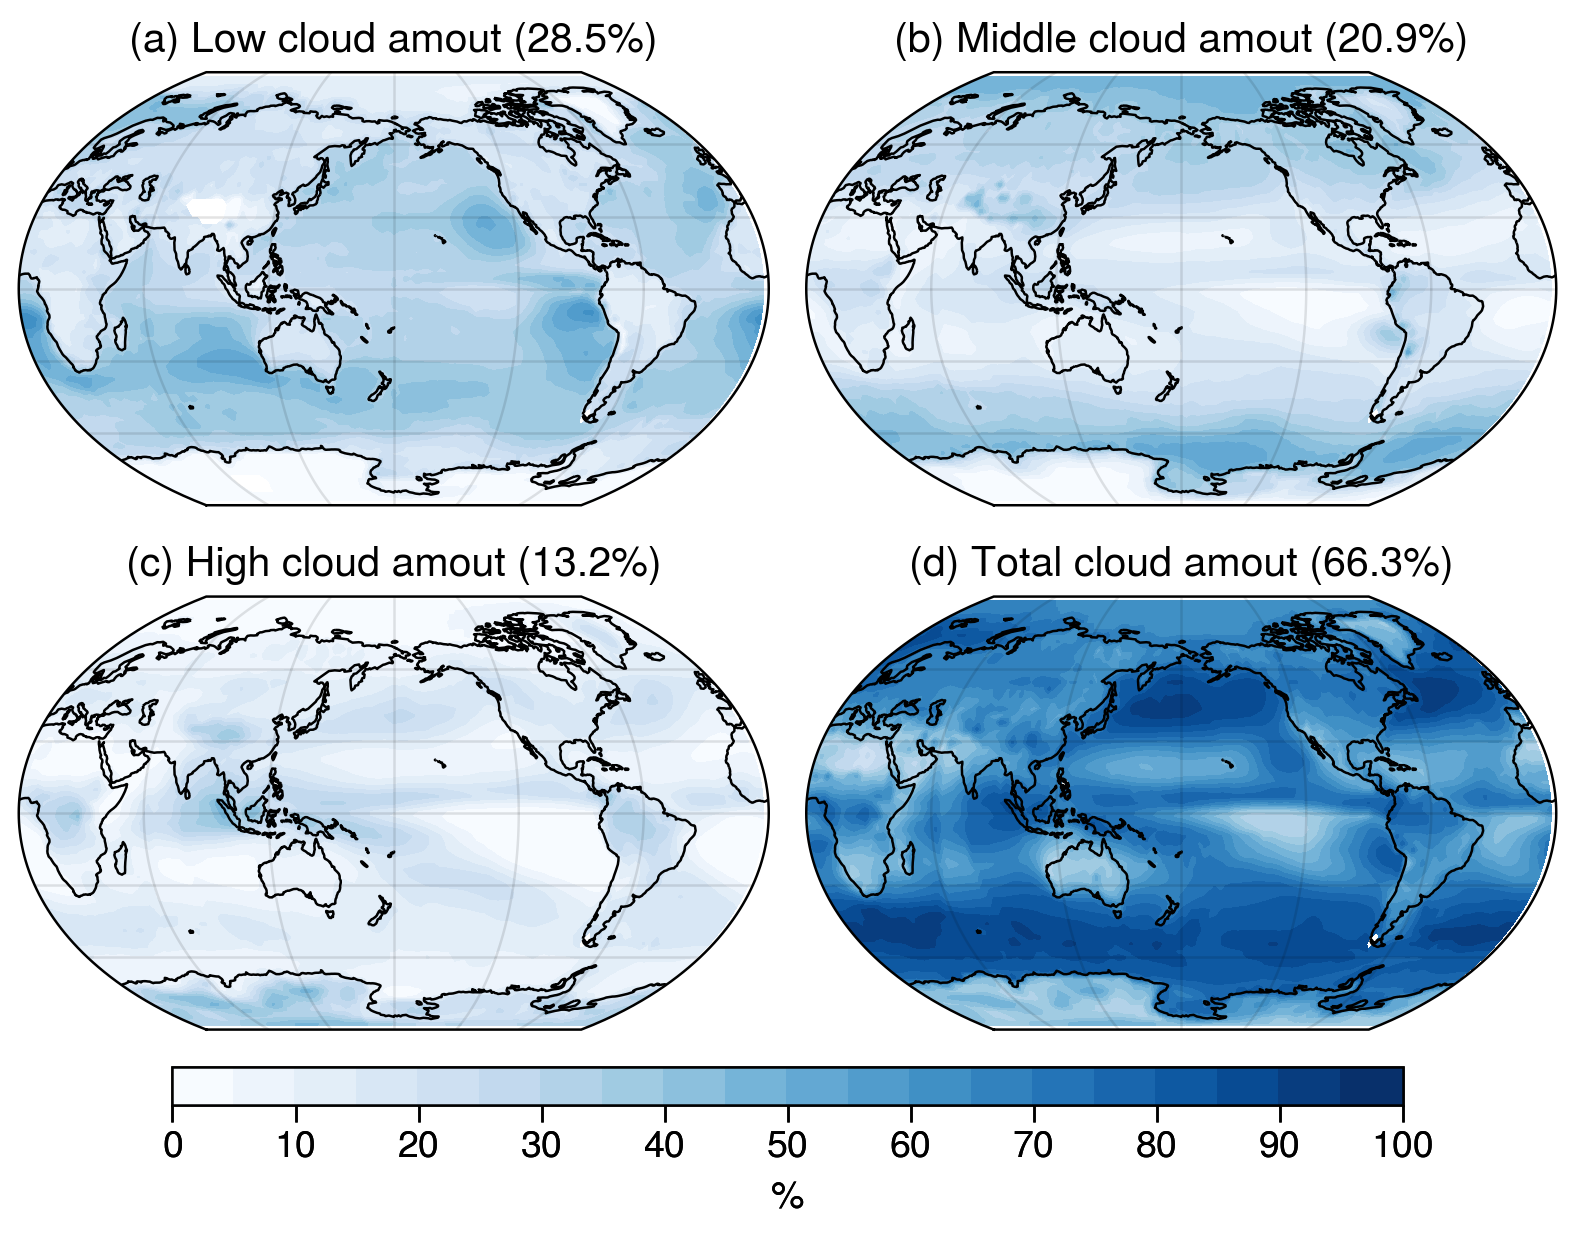
\includegraphics[width=0.7\linewidth]{{figs/literature_review/isccp_cldamt}.png}
	\caption[Distribution of annual-mean low, middle, high and total cloud amounts from ISCCP-H data set]{Distribution of annual-mean (a) low cloud amount (below 680 hPa), (b) middle cloud amount (440-680 hPa), (c) high cloud amount (above 440 hPa) and (d) total cloud amount from ISCCP H-series data set from 1984 to 2014. The global mean amounts are shown in titles.}
	\label{fig:cldamt_isccp}
\end{figure}

\begin{figure}[ht]
	\centering
	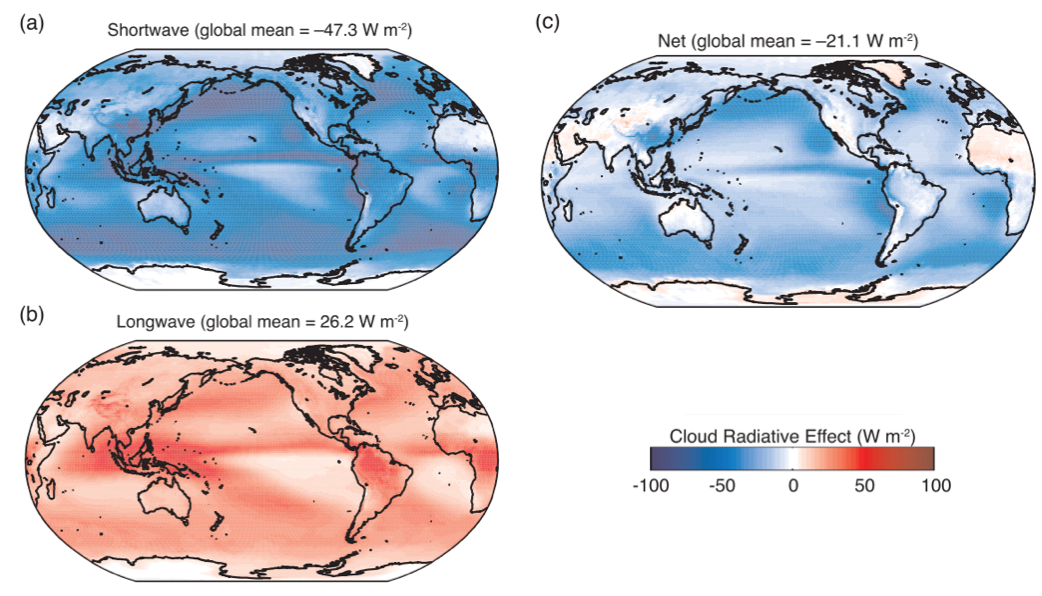
\includegraphics[width=0.8\linewidth]{{figs/literature_review/spatial_pattern_of_CRE_from_IPCC_ch7}.png}
	\caption[Distribution of annual-mean top of the atmosphere cloud radiative effects]{Distribution of annual-mean top of the atmosphere (a) shortwave, (b) longwave, (c) net cloud radiative effects averaged over the period 2001–2011 from the Clouds and the Earth’s Radiant Energy System (CERES) Energy Balanced and Filled (EBAF) Ed2.6r data set. Adapted from Fig. 7.7 of the Fifth Assessment Report (AR5) of the Intergovernmental Panel on Climate Change (IPCC) \citep{Stocker2013}.}
	\label{fig:CRE_from_IPCC}
\end{figure}

For shortwave CRE \index{Cloud radiative effect!shortwave}, we can write $R_{clr}=S_0\alpha_{clr}$ and $R_{cld}=S_0\alpha_{cld}$, such that \Eqref{eq:cre_new} becomes
\begin{equation}
    \mathrm{SWCRE} = S_0 C_{tot}(\alpha_{clr}-\alpha_{cld}),
    \label{eq:swcre2}
\end{equation}
where $S_0$ is solar constant, and $\alpha_{clr}$ and $\alpha_{cld}$ are clear-sky and all-sky albedo respectively. As the clear-sky albedo usually smaller than that in all-sky (i.e. $\alpha_{clr}<\alpha_{cld}$), the shortwave CRE is negative everywhere (\figref{fig:CRE_from_IPCC}a). This means clouds reflect more sunlight back to space than clear-sky conditions, and thus the shortwave effect of clouds is to cool the Earth. In addition, the magnitude of shortwave CRE increases with cloud fraction and albedo contrast between cloudy and clear conditions, as indicated by \Eqref{eq:swcre2}. For example, when comparing the distribution of total cloud amount (\figref{fig:cldamt_isccp}d) and shortwave CRE (\figref{fig:CRE_from_IPCC}a), we can find that the magnitude of shortwave CRE are large over regions of persistent cloudiness such as Southern Ocean, and are small over the regions where there is little cloud cover such as subtropical trade cumulus regions. In addition, the shortwave CRE generally has more negative values over ocean than over land, as the surface albedo over land is larger than ocean, thus the contrast between clear and cloudy albedo is smaller. The albedo of clouds can be derived from its optical depth (see \figref{fig:cld_optial_property}; \citealt{Liou1990remote}), a value determined by the combination of cloud macro-physical (e.g., cloud fraction and cloud water content) and micro-physical properties such as cloud droplet shape and size and cloud thermodynamic phase \citep{Stephens1978radiation}. This could bring lots of uncertainties and could be one possible reason that the shortwave cloud feedback is more uncertain than longwave component (see `Cloud$_{SW}$' and `Cloud$_{LW}$' columns in \figref{fig:zelinka_global_mean_fbks}; \citealt{Zelinka2020causes}).
 
For longwave CRE\index{Cloud radiative effect!longwave}, we can write $R_{clr}\approx \sigma T_{clr}^4$ and $R_{cld}\approx \epsilon_{cld}\sigma T_{cld}^4 +  (1-\epsilon_{cld}) \sigma T_{clr}^4$ based on Stefan--Boltzmann law, and after putting them into \Eqref{eq:cre_new}, the longwave CRE becomes
\begin{equation}
    \mathrm{LWCRE} \approx \epsilon_{cld} \sigma C_{tot}\left(T_{clr}^4-T_{cld}^4\right),
    \label{eq:lwcre2}
\end{equation}
where $\epsilon_{cld}$ is the emissivity of clouds, $\sigma$ is Stefan--Boltzmann constant, and $T_{cld}$ and $T_{clr}$ are emission temperature at cloudy and clear conditions, respectively. From \Eqref{eq:lwcre2} we can judge that longwave CRE is positive  (see \figref{fig:CRE_from_IPCC}b) as $T_{clr}>T_{cld}$. This indicates that clouds emit less longwave radiation to space than the clear-sky atmosphere, and thus can heat Earth. Additionally, the longwave CRE increases with cloud fraction, emissivity and the emission temperature contrast between clouds and clear-sky atmosphere, in which the last depends on the cloud top temperature. In fact, we can find the spatial patterns of longwave CRE (\figref{fig:CRE_from_IPCC}b) and high cloud amount (\figref{fig:cldamt_isccp}c) are similar. For instance, the longwave CREs are large over the areas with much high clouds, such as the Intertropical Convergence Zone (ITCZ); The longwave CRE is smaller where high clouds are rare, such as over the subtropical trade-wind cumulus region.

The net CRE\index{Cloud radiative effect!net} is the competing result of shortwave and longwave CREs, with the spatial pattern shown in \figref{fig:CRE_from_IPCC}c. Clearly, the large negative values over the regions with persistent low clouds (see \figref{fig:cldamt_isccp}a), such as Southern Ocean and subtropical eastern Pacific regions, as the shortwave CRE dominates over the longwave CRE in these regions. The net CRE over deep convective regions is near-zero due to the cancellation between shortwave and longwave components \citep[e.g.,][]{Wall2019net}.

In summary, different factors have impact on shortwave and longwave CREs, including both macrophysical (e.g., cloud fraction, cloud water content) and microphysical properties (e.g., cloud condensate shape and size). The net effect depends on its shortwave and longwave components, which have opposite signs and different magnitudes. For shortwave CRE, cloud amount and cloud albedo (or optical depth) are important factors to determine its strength; while for longwave CRE, the cloud amount (especially high cloud amount), cloud emissivity and the contrast of cloud top temperature with clear-sky atmosphere are important contributors to its magnitude. To better understand how cloud radiative properties change in response to the increase of greenhouse gas concentration, we need to investigate how these factors might change under global warming.

\subsection{Mechanisms of cloud feedback}
\label{sec:intro_cld_fbk_mechanism}

To fully understand cloud feedback is a challenging job, partly due to the diversity of clouds in climate system \citep{Ceppi2017,Zelinka2017}. For example, the clouds are located at different locations (e.g., low, middle and high clouds) and the cloud condensates are in different shapes or forms (such as liquid, ice or mixed phase), so they can affect the radiation in different ways. In addition, these clouds are usually controlled by different meteorological factors, therefore it is hard to predict the responses of clouds under climate change. Nevertheless, lots of efforts have been paid by previous studies to pin down the intermodel spread of cloud feedbacks \citep[e.g.,][]{Bony2004,Bony2005,Bony2006,Vial2013,Webb2015,Geoffroy2017,Zelinka2016insights,Myers2021,Ceppi2021observational}.

%\subsubsection{Cloud feedback in GCMs}

\begin{figure}[ht]
	\centering
	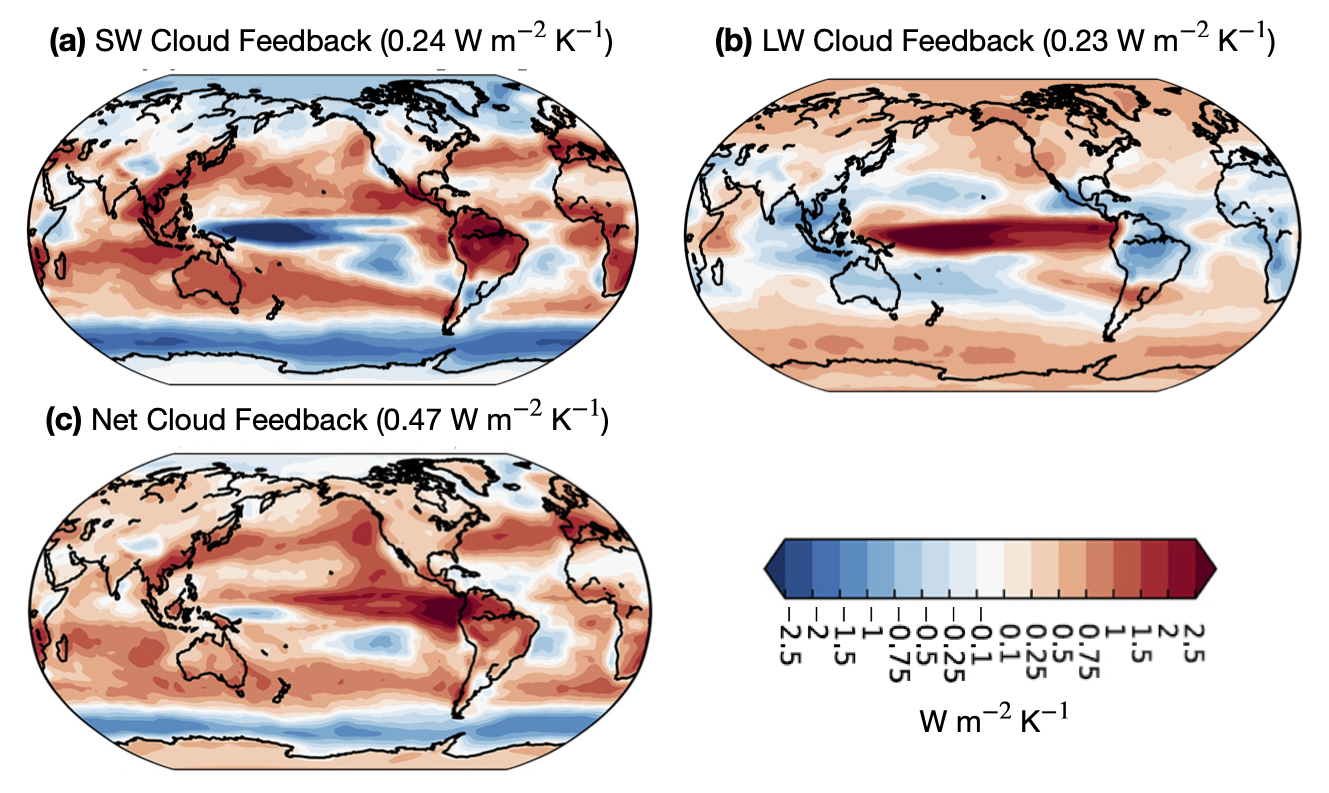
\includegraphics[width=0.9\linewidth]{{figs/literature_review/cld_fbk_cfmip12}.png}
	\caption[The multi-model ensemble mean spatial patterns of shortwave, longwave and net cloud feedbacks.]{Multi-model ensemble mean (a) shortwave, (b) longwave and (c) net cloud feedbacks for the first and second phases of Cloud Feedback Model Intercomparison Project \citep[CFMIP;][]{Webb2017cfmip} models, which are computed through the cloud radiative kernel technique. Adapted from Figs. 2, S5 and S6 of \cite{Zelinka2016insights} with permission of the John Wiley and Sons.}
	\label{fig:spatial_pattern_of_cld_feedbacks_Zelinka}
\end{figure}

The shortwave, longwave and net cloud feedbacks have been introduced in \secref{sec:individual_fbks}, and their spatial patterns simulated in the first and second phases of Cloud Feedback Model Intercomparison Project \citep[CFMIP;][]{Webb2017cfmip} models are shown in \figref{fig:spatial_pattern_of_cld_feedbacks_Zelinka}. The net cloud feedback is positive at nearly every location equatorward of 50$^\circ$, and negative in high latitudes such as Southern Ocean and Arctic region (\figref{fig:spatial_pattern_of_cld_feedbacks_Zelinka}c). When decomposing the net cloud feedback into shortwave and longwave components, we find that the shortwave cloud feedback is negative in lower and high latitudes, but positive over the subtropics. For instance, the shortwave cloud feedback is negative in Southern Ocean region (\figref{fig:spatial_pattern_of_cld_feedbacks_Zelinka}a). The longwave cloud feedback is positive in topical and high-latitude regions, and especially pronounced over tropical deep convection regions (\figref{fig:spatial_pattern_of_cld_feedbacks_Zelinka}b). The possible mechanisms for these feedbacks can be understood by further breaking down the cloud feedback into three categories (i.e., cloud amount, cloud altitude and cloud opacity feedbacks; \citealt{Zelinka2012computing2}) due to their different radiative properties. The features of net cloud feedback can be understood through the sum of these three different components \citep{Ceppi2017,Zelinka2017}, as we will explain below. %The possible reasons for the cloud feedback patterns in \figref{fig:spatial_pattern_of_cld_feedbacks_Zelinka} will be explained below.

% \begin{figure}[ht]
% 	\centering
% 	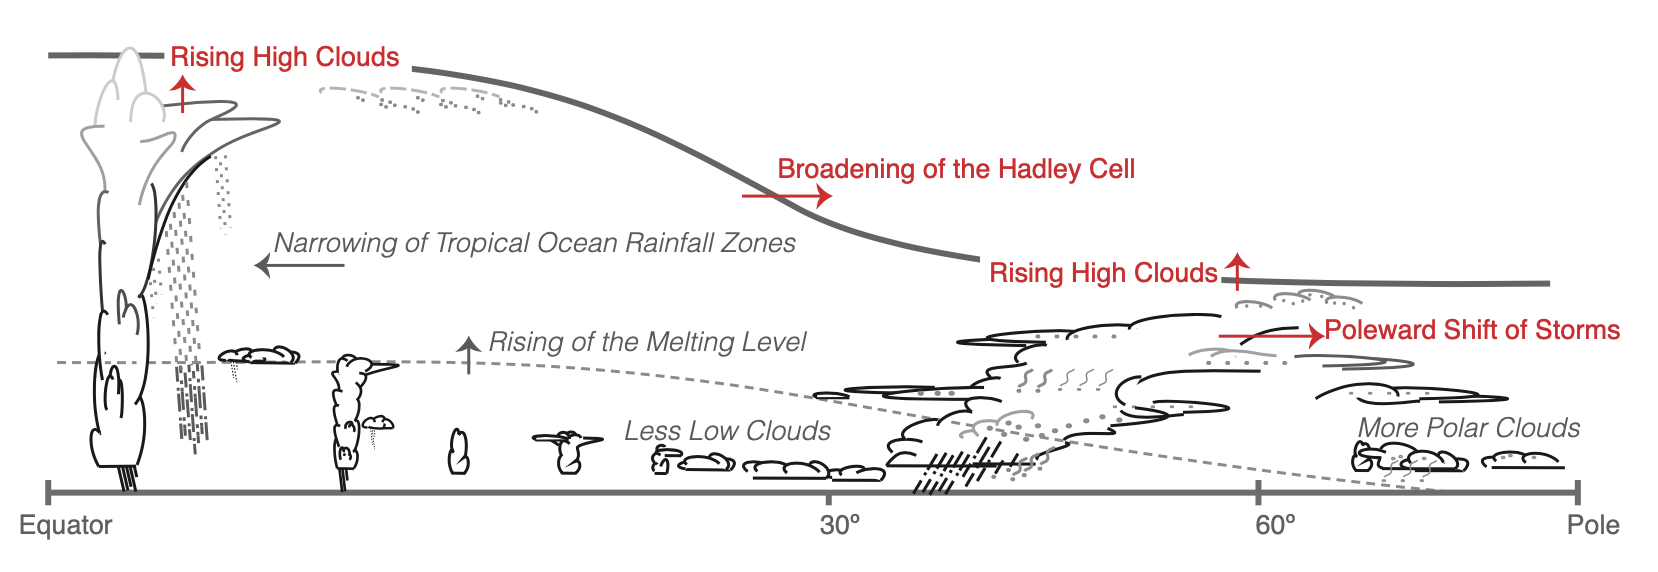
\includegraphics[width=0.9\linewidth]{{figs/literature_review/robust_cloud_responses_to_greenhouse_warming}.png}
% 	\caption[Robust Cloud responses to greenhouse warming from IPCC AR5.]{Robust cloud responses to greenhouse warming (those simulated by most models and possessing some kind of independent support or understanding). The tropopause and melting level are shown by the thick solid and thin grey dashed lines, respectively. Changes anticipated in a warmer climate are shown by arrows, with red colour indicating those making a robust positive feedback contribution and grey indicating those where the feedback contribution is small and/or highly uncertain. No robust mechanisms contribute negative feedback. Changes include rising high cloud tops and melting level, and increased polar cloud cover and/or optical thickness (high confidence); broadening of the Hadley Cell and/or poleward migration of storm tracks, and narrowing of rainfall zones such as the Intertropical Convergence Zone (medium confidence); and reduced low-cloud amount and/or optical thickness (low confidence). Confidence assessments are based on degree of GCM consensus, strength of independent lines of evidence from observations or process models and degree of basic understanding. Adapted from Figure 7.11 of IPCC AR5 \citep{Stocker2013}.}
% 	\label{fig:robust_cld_responses_ar5}
% \end{figure}

% Structure from Ceppi et al., 2017 review:
% What physical mechanisms are involved in the cloud response? To what extent are these mechanisms supported by theory, highresolution modeling, and observations?
% How well do GCMs represent these mechanisms, and what parameterizations does this depend on?
% What explains the intermodel spread in cloud responses?

\subsubsection{Altitude feedback}
\index{Altitude feedback}

As introduced in \secref{sec:CRE_intro}, high clouds have much larger longwave cloud radiative effect due to their colder cloud top temperature. As clouds get higher, they will have lower temperature and emit less infrared radiation to space. Therefore, the increase in cloud altitude has a warming effect on climate by reducing the outgoing longwave radiation. 

One robust cloud change under global warming is the positive longwave cloud feedback in tropical regions (\figref{fig:spatial_pattern_of_cld_feedbacks_Zelinka}b), which is believed to be related to the rising of high clouds (e.g., \citealt{Wetherald1988cloud}).  
The positive longwave cloud altitude feedback can be explained by the fixed anvil temperature (FAT) hypothesis, which is first proposed by \cite{Hartmann2002FAT}, and used by lots of later studies \cite[e.g.,][]{Kuang2007,Zelinka2010longwave,Yoshimori2020fixed}. The FAT theory holds that the isotherms move up and convection deepens in tropical region as climate warms, but the cloud-top temperature of anvils remains approximately constant. In this case, according to \Eqref{eq:lwcre2}, the cloud-top temperature do not warm in step with the surface warming and the OLR keeps relatively constant, so the tropics become less efficient at radiating the heat away and more heat would be trapped within the Earth, indicating that high clouds act as a positive feedback on climate under global warming.

\subsubsection{Optical depth feedback}
\index{Optical depth feedback}

Another robust cloud change in response to increasing concentrations of CO$_2$ is the cloud phase change from the middle to high latitudes \citep[e.g.,][]{Storelvmo2015cloud,Ceppi2016mechanisms,Tan2016observational,McCoy2016relationships}. As the melting level shifts upward and poleward in response to warming, the ice condensate in mixed-phase clouds (i.e., containing both liquid and ice condensate) melts into liquid water. That is to say, the occurrence of liquid water in clouds should increase relative to ice. Therefore, for a fixed cloud condensate amount, this leads to the increase of cloud optical depth \citep{Stephens1978radiation}, due to the smaller effective radius of liquid droplets \citep{Stubenrauch2013}. In addition, given the ice cloud droplets are larger than liquid clouds, ice clouds tend to precipitate more efficiently. That is to say, the cloud life time is longer after cloud phase changing from ice to liquid, making the liquid clouds persist longer than ice clouds and a further optical thickening of the cloud \citep{Storelvmo2015cloud,Ceppi2016mechanisms}. Therefore, more shortwave radiation would be reflected back to space due to this optical depth change, resulting in a negative shortwave feedback \citep[e.g.,][]{Zelinka2012computing1,Zelinka2012computing2,Zelinka2013contributions,Ceppi2016mechanisms,Tan2016observational,McCoy2016relationships,Zelinka2020causes,Bjordal2020equilibrium}. As this phase change mechanism can only operate below freezing, its occurrence in low clouds is evident in middle and high latitudes as shown in \figref{fig:spatial_pattern_of_cld_feedbacks_Zelinka}a \citep{Ceppi2017}. 

% This negative mechanism can also be understood through \Eqref{eq:swcre2}: more liquid water in clouds increases the optical depth and albedo, and thus a much negative shortwave CRE, if other factors such as cloud amount, solar constant and clear-sky albedo remain unchanged.

However, this negative optical depth feedback from hydrometeor phase change is perhaps overestimated in CMIP5 models due to the poor representation of supercooled liquid cloud in mixed-phase clouds \citep{Tan2016observational,Frey2018influence}. Too much present-day ice in mixed-phase clouds leads to stronger negative optical depth feedback under global warming. This bias is partly mitigated in CMIP6 models, and thus the negative optical depth feedback over middle to high latitudes weakens, which leads to the increase in net cloud feedback and in ECS in CMIP6 models \citep[e.g.,][]{Zelinka2020causes,Bjordal2020equilibrium}. But we should also notice that this cloud phase change would make the precipitation less likely \citep[e.g.,][]{Korolev2017mixed}, hence increasing the cloud lifetime and bringing a negative feedback. But as the warm clouds precipitate too readily in CMIP models, this negative cloud lifetime feedback is underestimated in current GCMs and the simulated ECS might be higher than it should be \citep{Mulmenstadt2021underestimated}.

\subsubsection{Cloud amount feedback}
%Compared to the longwave cloud feedback of high anvil clouds, the shortwave cloud feedback still ``lacks a well-accepted theoretical basis" \citep{Stocker2013}.  %From then on, many studies have tried to understand the causes of shortwave cloud feedback.
%Compared to the positive high clouds feedback and
%The most uncertain part of cloud feedback is related to the low cloud amount changes under global warming \citep{Stocker2013}.
The feedback induced by the cloud amount change is different for different cloud types. Specifically, the warming induced
by increase of high, thin clouds usually leads to a positive feedback. The reason is that the optical depth of these high,
thin clouds is typically small, thus having little impact on the shortwave radiation. However, such clouds can absorb the longwave radiation and thus constitute a strong greenhouse effect. This can also be inferred from \Eqref{eq:lwcre2}: the increase of high cloud amount leads to the rise of longwave CRE, which is a heating effect on climate. In contrast, the warming induced increase in the amount of low clouds (especially the opaque ones) brings a negative feedback as less sunlight can reach the surface, thus a cooling effect. As shown in \Eqref{eq:swcre2}, the increase of cloud amount (especially the low opaque clouds) strengthens the magnitude of shortwave CRE, which is a cooling effect on climate. Currently, there is still lack of a well-accepted theoretical basis for the possible changes of low cloud amount, and the GCMs have low confidence in simulating their changes under global warming \citep{Stocker2013}.

%For different cloud types, the change in cloud amount has different effect on climate. According to \Eqref{eq:lwcre2}, the increase of cloud amount, especially high cloud amount, leads to the rise of longwave CRE, which is thus a heating effect on climate. Similarly, the increase of cloud amount (especially the low cloud amount) also strengthens the magnitude of shortwave CRE according to \Eqref{eq:swcre2}, but it has cooling effect on climate as the sign of shortwave CRE is negative. Naturally, reduced low cloud amount has a warming effect to climate as more incoming solar radiation can reach the surface. 

%pattern effect
The low cloud amount feedback in GCMs is dominated by the response of boundary-layer cloud types at low latitudes: stratus, stratocumulus, and cumulus clouds \citep{Ceppi2017}. Although they cover a relatively small fraction of Earth, the low clouds such as stratus and stratocumulus have relatively large shortwave CREs, so that even small changes in their coverage may have significant regional and global impacts \citep[e.g.,][]{Schneider2019}. The formation and dissipation of low clouds are controlled by the differences between the supply of moisture from the surface and the mixing of relatively dry air in free troposphere. Observations have shown a strong relationship between inversion strength at the top of the planetary boundary layer and cloud amount \citep{Gordon1992,Klein1993,Wood2006}. Stronger inversion weakens the mixing between moisture boundary layer and dry free troposphere aloft, so more moisture is trapped below the inversion layer, thereby favoring more low-level clouds \citep[e.g.,][]{Qu2014,Qu2015positive,Scott2020}. In contrast, the increase in sea surface temperature (SST) leads to the higher temperature and saturation water vapor pressure in the boundary layer, which can weaken the inversion strength if the temperature in the free troposphere remains constant. In this case, the in-cloud latent heating enhances the turbulance and entrainment of the drier air from aloft into the boundary layer, thus resulting in the reduction of cloudiness in low level \citep[e.g.,][]{Rieck2012, Webb2013coupling, Qu2014, Bretherton2015, Brient2016,Myers2016,Ceppi2017relationship,Scott2020}. This mechanism is not only found in large-eddy simulations \citep{Bretherton2015}, but also supported by some GCM simulations \citep[e.g.,][]{Zhang2013CGILS,Myers2016} and recent low cloud constraints constructed from satellite observations \citep{Scott2020,Myers2021}. The inversion strength and SST are two major meteorological factors to determine the observed natural variability of low cloud amount \citep[e.g.,][]{Zhou2016,Cesana2021}. In addition, other factors such as the relative humidity in the free troposphere, the strength of large-scale subsidence, warm/cold temperature advection and surface wind speed also have impacts on the cloudiness at low troposphere, but their contributions are relatively small \citep[e.g.,][]{Bretherton2015,Myers2016,Scott2020}.
%Specifically, (1) weaker subsidence under global warming can raise the cloud tops and make the cloud layer thicker, thereby a negative feedback. (2) If the relative humidity in free troposphere is large, the moisture contrast between boundary layer and free atmosphere aloft is small, then the cloud-top entrainment drying is weaker, which thus favors more low-level clouds (negative feedback). At the same time, more free-tropospheric moisture emits more downwelling longwave radiation, which can weaken cloud-top radiative-cooling and the overturning circulations that mix moisture up from the surface, thereby favoring less low-level cloud (postive feedback). (3) Low-level advection from cold to warm SST brings relatively cool and dry air over warmer water, which triggers enhanced upward turbulent fluxes of heat and moisture from the sea surface, providing a strong source of moisture for cloud formation, therefore a negative feedback. Conversely, low-level airflow from warm to cold SST brings relatively warm and moist air over cooler water, which stabilizes the boundary layer and cuts off clouds from the surface moisture supply and thus a positive feedback. (4) Stronger winds increase evaporation from the sea surface and promote deepening of the boundary layer, favoring the formation of low clouds and thus a negative feedback. In summary, the change of low cloud amount could be from the net effect of these competing processes, but studies found the contributions from these factors to low cloud amount change in GCMs are relatively limited compared to inversion strength and SST \citep{Myers2016,Scott2020}.

 Moreover, previous studies also find that low cloud changes depend not only on local SST changes, but also on some remote effects \citep[e.g.,][]{Zhou2015,Zhou2016,Zhou2017,Mauritsen2016clouds,Andrews2018}. For example, \cite{Zhou2017} analyzed the dependence of global cloud feedback on the spatial pattern of SST change with a Green's function approach, and found that warming in tropical ascent regions increases the free-tropospheric temperature throughout the tropics, thereby enhancing the inversion strength over remote regions and inducing positive change in global low cloud amount and negative CRE anomalies; while the warming in the tropical subsidence or extratropical regions only causes local decrease in low cloud amount and positive change in CRE. These results suggest that the low cloud amount feedbacks could be different due to the differences in SST warming patterns, the so called `pattern effect' \citep[e.g.,][]{Dong2020intermodel}.

In CMIP models, the low cloud amount feedback is the largest single contributor to the intermodel spread of net cloud feedback \citep{Bony2005,Caldwell2016quantifying,Zelinka2016insights}. It has been suggested that the different convective parametrizations play important roles in driving the spread of low cloud amount feedback and climate sensitivity \citep[e.g.,][]{Gettelman2012,Zhao2014investigation,Sherwood2014spread}, but \cite{Webb2015} found that the range in cloud feedbacks among the CFMIP models did not change substantially when convective parametrizations were switched off, implying that some non-convective processes must also contribute substantially to the overall intermodel spread of cloud feedback. Also, previous study such as \cite{Qu2014} has suggested that models with different type of cloud schemes may predict opposite cloud cover changes under global warming in several marine stratocumulus regions in subtropical ocean region off the west coasts of continents. Subsequently, \cite{Geoffroy2017} implemented six different diagnostic cloud schemes found in CMIP models into two test-bed climate models, and found that roughly half of the multi-model spread in the cloud feedback in stratocumulus regions could be reproduced by changing the stratiform cloud scheme alone, suggesting that different stratiform cloud schemes play an important part in the spread of cloud feedback, both in stratocumulus cloud regions and globally. From these studies we can find that the intermodel spread in cloud feedback in GCMs depend not only on cloud scheme (i.e., how clouds are represented in GCMs) itself \citep[e.g.,][]{Qu2014,Geoffroy2017}, but also on the interaction between clouds and various physical process such as shallow convective mixing, turbulence and radiation \citep[e.g.,][]{Vial2016coupling}.

% Other factors controlling cloud feedback
% Cloud - circulation coupling?

\section{Cloud scheme}
\label{sec:cld_scheme_history}
\index{Cloud scheme}

%\subsection{Overview}
\begin{figure}[ht]
	\centering
	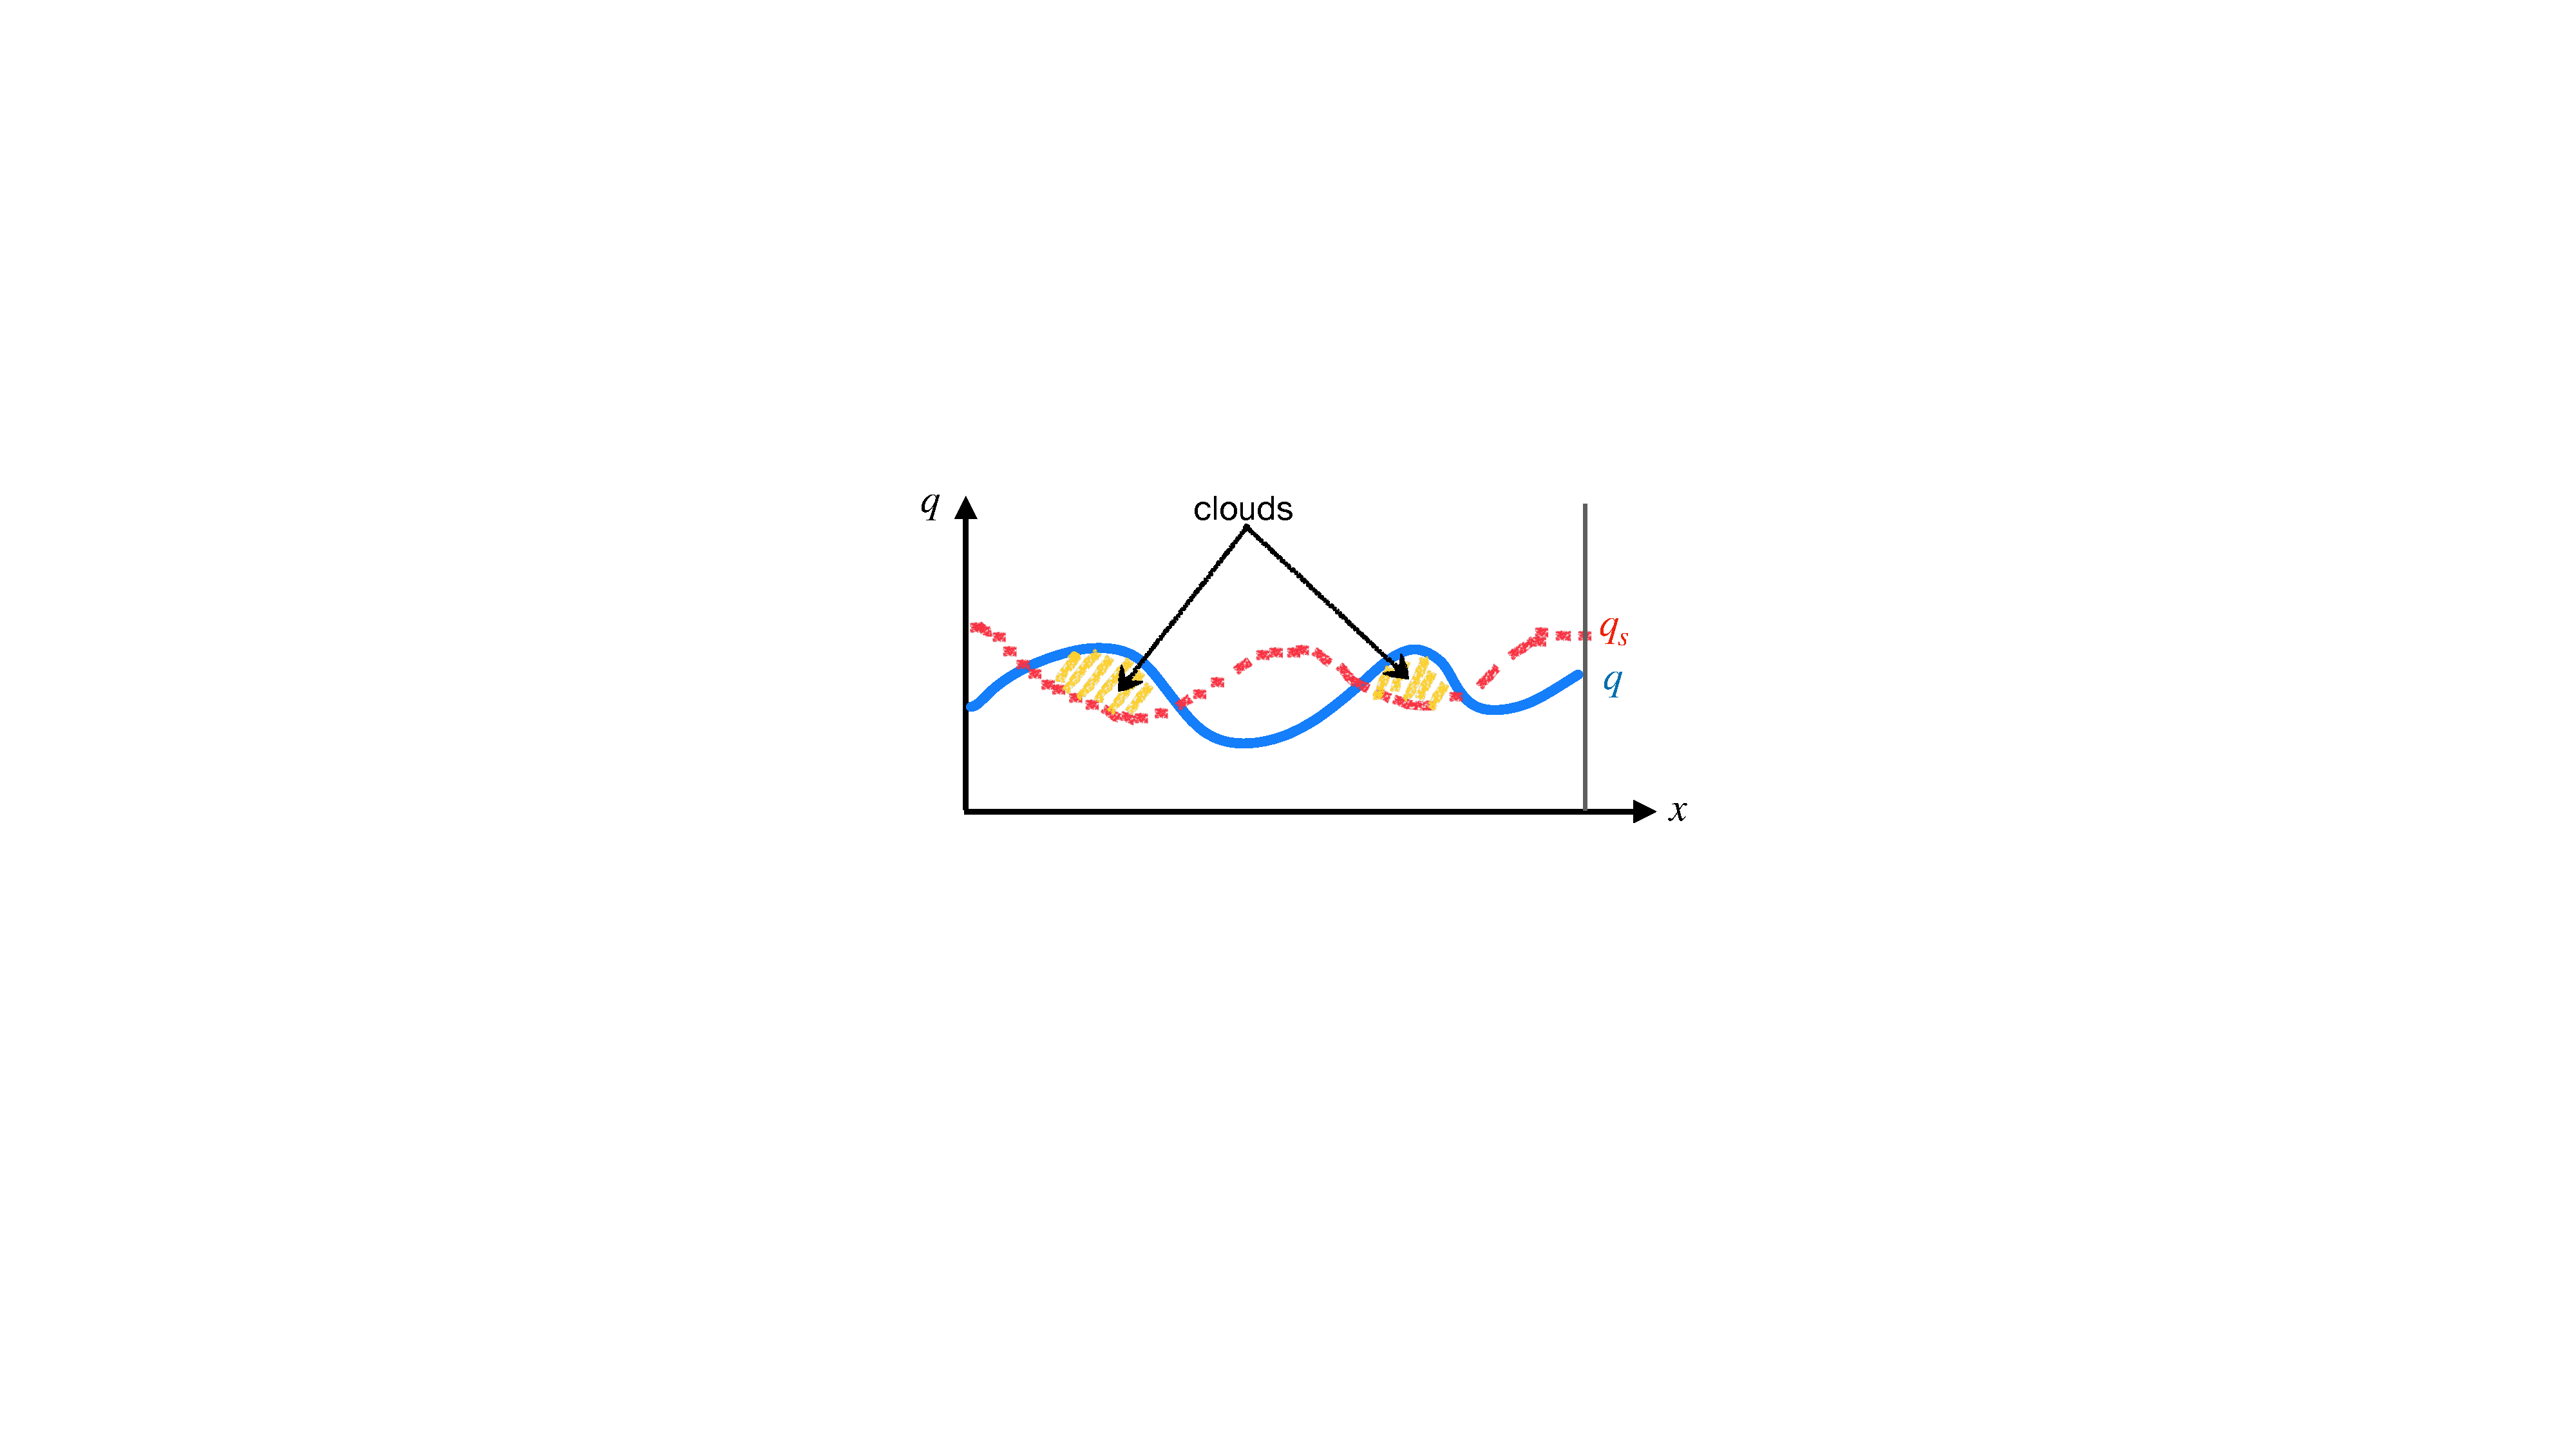
\includegraphics[width=0.5\linewidth]{{figs/literature_review/Schematic_partial_cloud_cover_in_gridbox}.pdf}
	\caption[Schematic showing that partial cloud cover in a grid box (1D) when temperature or humidity fluctuations exist]{Schematic showing that partial cloud cover in a grid box (1D) when temperature or humidity fluctuations exist. The blue line shows humidity and the red dashed line indicates saturation mixing ratio of the grid box. The shaded regions are cloudy parts as the humidity exceeds the saturation mixing ratio.}
	\label{fig:schematic_partial_clouds}
\end{figure}

At present the typical horizontal resolution of the GCMs is 50-200km, but the clouds usually involve the air motions in mesoscale and convective scale \citep{Houze2014}, which are usually in sub-grid scale both horizontally and vertically, implying that cloud processes are hard to be explicitly resolved by the GCMs. In this case, the ``parameterization" becomes a practical way to build cloud schemes. The parameterization is to represent the effects of the smaller-scale processes (turbulence, cloud microphysics, convection, etc.) in terms of the large-scale states (such as velocity, temperature, pressure, humidity) \citep{Randall2003}, which could be seen as a way to find potential relationships between the unknown and known variables \citep{Randall1989}.

\subsection{Relative humidity schemes}
\index{Cloud scheme!RH scheme}
Previous studies have investigated various ways to represent clouds in climate models. For example, \cite{Holloway1971} prescribed the clouds externally with climatological data without dynamic interplay with the other components of the model. Some early modelling studies made the assumption that a grid box in the model is either fully saturated or totally unsaturated. However, this assumption is not reasonable enough as the humidity can distribute unevenly within a grid box, suggesting that condensation can occur even the relative humidity is less than 100\%, as shown in \figref{fig:schematic_partial_clouds}. A general idea is to link the cloud cover with the relative humidity (RH), as one can expect that the amount of condensation would increase with the increase of mean humidity of the model grid box, which is the basis for some diagnostic methods.

Diagnostic schemes predict the cloudiness based on the model variables empirically or statistically. In these schemes, the clouds can be linked to atmospheric outputs such as relative humidity, vertical velocity and static stability, among which the linear relationship between cloud fraction against RH could be simplest one. For example, \cite{Smagorinsky1960} found empirically that non-convective cloud amount correlated with the average relative humidity in the respective layers, arguing that the non-precipitating condensation depends only on the accumulated history of vertical motion, which can be reflected by the humidity. \cite{Ricketts1973} obtained roughly linear relationship between cloud amount and observed relative humidity but commented that the relationship is somewhat indefinite.

Water vapor generally distributes heterogeneously in the grid box, so the averaged RH within a box should be less than 1 for a partial coverage of clouds (\figref{fig:schematic_partial_clouds}). Previous studies usually adopt the critical relative humidity $RH_{crit}$ as the minimum threshold for clouds to form, which is often left as a free parameter that can be tuned during model development \citep[e.g.,][]{Hourdin2017,Kay2012,Mauritsen2012}. For example, \cite{Sundqvist1978} and \cite{Sundqvist1989} find that cloud fraction can be rewritten as a function of critical RH by assuming the water vapor is uniform distributed within the grid box. In general, $RH_{crit}$ decreases with height, but will vary according to different types of clouds. Although the $RH_{crit}$ does not have clear physical meaning, it can be used to modify the cloud amounts in different locations. For example, one can increase $RH_{crit}$ asymptotically to nearly unity to prevent the unrealistic circus clouds \citep{Sundqvist1989}. 

As a unique predictor, RH is very simple and useful to diagnose the cloudiness, and it is still widely used in GCMs \citep[e.g.,][]{Gordon1992,Park2014,Pope2000}. However, it is not valid for all the cases. As we can see, some studies also made use of other variables to diagnose the cloudiness. For instances, \cite{Xu1996} developed a semi-empirical scheme to determine the stratiform cloud fraction based on grid-averaged mixing ratio of condensate (cloud water and cloud ice) and RH. As for the scheme provided by \cite{Slingo1987}, both the RH and vertical velocity were taken into account, in which different empirical relations were used for different clouds including low, middle, high and convective clouds.

In summary, the methods based on relative humidity and other predictors are useful to diagnose the cloudiness, which ensures that the clouds can form before the grid box get saturated. One problem for the diagnostic methods is that in most cases the cloud condensate has to be diagnosed or prognosed via other methods \citep[e.g.,][]{Zhang2003,Park2014}, which could lead to some inconsistencies between cloud fraction and cloud condensate \citep[e.g.][]{Gregory2002,Tompkins2005}.

% \begin{figure}
% 	\vspace{-0.3cm}
% 	\centering
% 	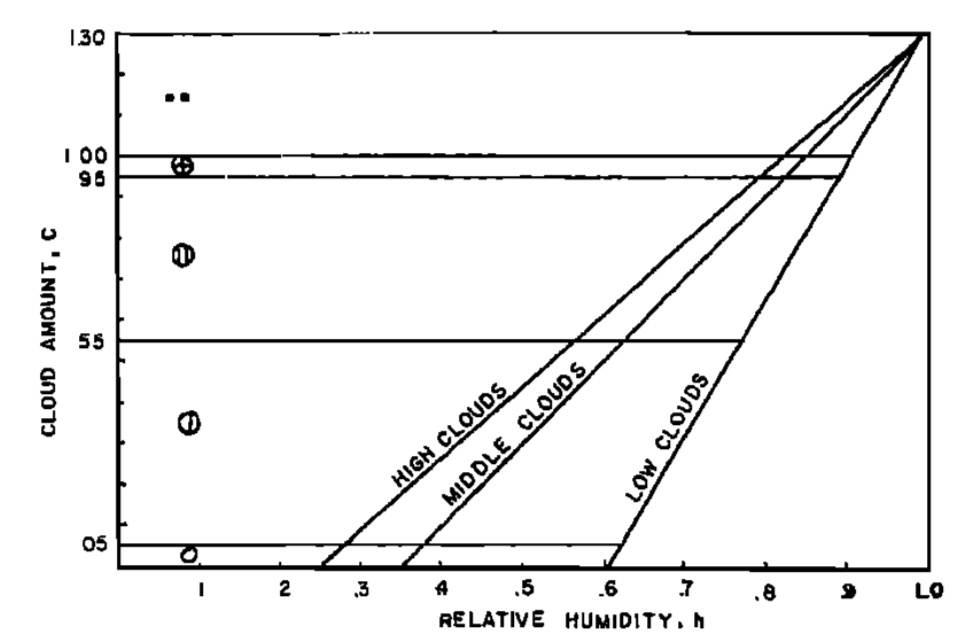
\includegraphics[width=0.6\linewidth]{{figs/literature_review/Smagorinsky1960}.png}
% 	\caption{Empirically determined relation of mean relative humidity $h$ in the layers 1000-800mb, 800-550mb and 550-300mb with cloud amount $c$ classed as low, middle and high clouds. Adapted from Figure 1 of \cite{Smagorinsky1960}.}
% 	\label{fig:Smagorinsky_RH_cld}
% \end{figure}

\subsection{Statistical schemes}
\label{sec:PDF_cld_scheme}
\index{Cloud scheme!statistical or PDF scheme}

In contrast, the prognostic approach \citep[e.g.,][]{Tiedtke1993} is to explicitly calculate the clouds related variables, such as cloud water content, in order to pursuing a unification of all clouds processes, which is more realistic in some degree and requires more physical basis and interactions with other parts of the models. Another widely used cloud prediction method is statistical scheme, in which the cloud fraction and in-cloud liquid water/ice are determined based on the assumed probability distributions of subgrid variability of thermodynamic properties. As the cloud related variables such as moisture and temperature are not the same everywhere but distributed randomly within the grid box, it is natural to assume that the cloud cover depends on the distribution of moisture, sometimes on the joint distribution of moisture and temperature. As shown in a very early work, \cite{Sommeria1977} gave up the assumption that a grid is either entirely saturated or unsaturated in the climate models and proposed the idea to use the statistical distribution of moisture within the grid box. In this case, given the probability distribution function (PDF) of the total water ($q_t$ is the mixing ratio) in grid box, the cloud fraction ($CF$) can be calculated as 
\begin{equation}
    CF=\int_{q_s}^{\infty}\text{PDF}(q_t)\operatorname{d}q_t,
\end{equation}
and the cloud water content ($q_c$ is the mixing ratio of cloud water) is
\begin{equation}
    q_c=\int_{q_s}^{\infty}(q_t-q_s)\text{PDF}(q_t)\operatorname{d}q_t,
\end{equation}
where $q_s$ is the saturation mixing ratio in both formulations.

However, the shapes of subgrid-scale PDF of total water specific humidity, saturation deficit, or a combined variable of liquid water and potential temperature are difficult to determine due to limitation of observational data, so sometimes the model data are also used \citep{Bony2001}. Additionally, many different PDF forms have been proposed in the previous studies. For example, \cite{LeTreut1991} made use of the uniform distribution of total water in the grid box to calculate the cloud cover and liquid water content. Other symmetrical distributions, such as Gaussian distribution \citep{Sommeria1977}, triangular distribution \citep{Smith1990} and skewed distributions, such as lognormal distribution \citep{Bony2001} and beta distribution \citep{Tompkins2002}, have also been employed in numerical models. However, there are also some problems in the distributions. For example, the Gaussian distribution is unbounded, indicating that the maximum cloud condensate mixing ratio might approach infinity, and cloud cover is always large than zero \citep{Tompkins2002}. In general, complicated forms of the PDF need more parameters to fit. But due to the limitation of the data, it is possibly hard to validate the distributions. Linking the statistical cloud scheme to other physical processes seems a promising way to improve cloud simulations. For example, \cite{Qin2018} developed a Gaussian PDF cloud scheme with the PDF variance diagnosed from the turbulent
and shallow convective processes, which could improve the simulation of low marine clouds and alleviate double Intertropical Convergence Zone (ITCZ) problem \citep{Qin2018alleviated}.

%The statistical cloud schemes may have better performance than the diagnostic ones, but considering the fact that there is no clouds scheme in Isca currently, it would be useful to implement the simple diagnostic schemes in Isca first, which can be seen as the first step to implemented a hierarchy of cloud schemes.

\subsection{Relationship between relative humidity and statistical schemes}

As discussed in previous section, one has to determine the expression of sub-grid variance (i.e. second order moment) or other higher-order moments in the statistical schemes. In doing so there are two general practices in current studies. The simple case is to use the time-invariant variance \citep[e.g.,][]{Sundqvist1978,Smith1990}, and the other approach is to employ time varying variance, which are usually obtained from other physical processes such as boundary layer scheme or shallow convection schemes \citep[e.g.,][]{Qin2018}. The second case usually provides a more realistic link between clouds and other physical processes \citep{Tompkins2002}. 

Note that there is no distinction between the RH schemes and statistical schemes, although they seem different in forms. As a matter of fact, if the subgrid variance in a statistical scheme is assumed to be time-invariant, it can be reduced to a RH scheme \citep{Tompkins2002,Tompkins2005}. The key is to link the variance with the critical relative humidity. That is to say, critical RH value can reflect the level of sub-grid variance in RH schemes \citep{Quaas2012}. Larger critical RH value means the lower subgrid variability and vice versa. For example, the RH scheme from \cite{Sundqvist1978} can be derived by assuming a uniform distribution of total water mixing ratio within a grid box, in which the variance is assumed a constant fraction of the saturation water vapor mixing ratio, and this constant is associated with critical RH value (see Appendix A of \cite{Quaas2012} for a full derivation). Another example is the triangular distribution used by \cite{Smith1990} and \cite{Park2014}, they also obtain the equivalent RH formulation by assuming the variance is related to critical RH. As pointed by \cite{Tompkins2002}, the parameterizations such as \cite{Xu1996}, in which cloud fraction is related to RH and cloud condensate, can be viewed as manifestations of the statistical schemes although where the actual PDFs of total water are not known. %, but the time-mean statistics of its integral are.

%\section{Research questions and thesis outline}
\section{Thesis outline}
\label{sec:thesis_layout}

The goal of this thesis is to understand the climate feedbacks with simple models, and the thesis is arranged as follows:

\chapref{ch:introduction} introduces the motivation, backgrounds and outline of this study. The backgrounds include the basic ideas of Earth's radiation budget, climate feedbacks, cloud radiative effects and their feedback mechanisms, and a brief introduction of climate parameterization schemes.

 The data and methods used in the thesis are presented in \chapref{ch:methods}. The data sets include the satellite observations about clouds and radiation, and other climate variables, such as temperature, relative humidity and vertical velocity, from the reanalysis. The methodology part first gives a brief introduction of Isca model, then presents the methods used in the thesis to calculate and decompose the cloud feedbacks. Finally, several low cloud proxies used in \chapref{ch:simple_cld_scheme} are listed for reference.
 % This should have two parts: First is about how to employ kernel method in Isca to estimate Planck, lapse rate, water vapor feedbacks for gray and RRTM radiation schemes; Second is to compare the methods to calculate the cloud feedback.

\chapref{ch:polaramplification} mainly presents the results from polar amplification of surface temperature change in aquaplanet simulations. In this chapter, the contributions from different climate feedbacks, forcing and heat transport are quantified through the decomposition method. The major conclusion is that the local lapse rate feedback and Planck feedback (plus heat transport) play important roles in determining the warming structure in polar region.

\chapref{ch:simple_cld_scheme} focuses on the parameterization of simple cloud scheme and the evaluation of its simulation of cloud climatology. These include the parameterization of the cloud fraction and cloud optical properties, simulation setup and the comparison of the simulated cloud fraction, radiative flux and cloud radiative effect with observations and CMIP5 models. The comparison consists of the spatial pattern, zonal mean structure and seasonal cycle. %Basically, this chapter is modified from the GMD manuscript. The content to be added is the sensitivity of the scheme to horizontal and vertical resolutions.

The topics of \chapref{ch:cld_fbk} are cloud feedback and its uncertainty. First, the cloud feedback simulated from the simple cloud scheme is evaluated. The spatial patterns of longwave, shortwave and net cloud feedbacks, as well as their components such as cloud amount, altitude and optical depth feedbacks, will be investigated and compared with the CMIP models. The possible reasons for the feedback features are to be explored. Then the results from perturbed parameter ensemble (PPE) will be analysed. The cloud feedback spread from the PPE simulations will be checked to see if they could `reproduce' such spread in CMIP models. The causes to the cloud feedback spread in Isca PPE will be investigated. Base on these results, which parameter or process is more sensitive would be analysed. Finally, the implications for equilibrium climate sensitivity will be discussed.

Finally, \chapref{ch:conclusion} summarizes the major contents and conclusions of the thesis, and discusses the possible future work.
